\documentclass[11pt,a4paper]{report}

% ---------- Packages ----------
\usepackage[utf8]{inputenc}
\usepackage[T1]{fontenc}
\usepackage{graphicx}
% ---------- Simpler, more readable font ----------
\usepackage{lmodern}
\usepackage[sfdefault]{noto}
\usepackage[T1]{fontenc}
\usepackage{geometry}
\geometry{margin=1in}
\usepackage{fancyhdr}
\usepackage{titlesec}
\usepackage{booktabs}
\usepackage{longtable}
\usepackage{array}
\usepackage{listings}
\usepackage{xcolor}
\usepackage{hyperref}
\usepackage{amsmath}
\usepackage{amssymb}
\usepackage{tikz}
\usetikzlibrary{shapes,arrows.meta,positioning,automata}
\usepackage{caption}
\usepackage{enumitem}
\usepackage{csquotes}
\usepackage{tocloft}

% ---------- Bibliography ----------
\usepackage[backend=biber,style=numeric,sorting=none]{biblatex}
\addbibresource{references.bib}

% ---------- Listings style ----------
\definecolor{codebg}{RGB}{245,245,245}
\definecolor{codekeyword}{RGB}{0,0,180}
\definecolor{codecomment}{RGB}{95,140,95}
\definecolor{codestring}{RGB}{160,20,20}

\lstdefinestyle{codestyle}{
    backgroundcolor=\color{codebg},
    commentstyle=\color{codecomment},
    keywordstyle=\color{codekeyword}\bfseries,
    stringstyle=\color{codestring},
    basicstyle=\ttfamily\footnotesize,
    breakatwhitespace=false,
    breaklines=true,
    captionpos=b,
    keepspaces=true,
    numbers=left,
    numbersep=5pt,
    numberstyle=\tiny\color{gray},
    showspaces=false,
    showstringspaces=false,
    showtabs=false,
    tabsize=2,
    frame=single,
    rulecolor=\color{gray!40}
}
\lstset{style=codestyle}
\lstdefinelanguage{JavaScript}{
  keywords={function, return, if, else, for, while, const, let, var, new, this, export, import, from, default, class, extends, try, catch, throw, async, await, static},
  keywordstyle=\color{codekeyword}\bfseries,
  comment=[l]{//},
  morecomment=[s]{/*}{*/},
  string=[s]{"}{"},
  stringstyle=\color{codestring},
  sensitive=true
}
\lstdefinelanguage{PHP}{
  keywords={function, return, if, else, elseif, for, while, foreach, as, require_once, echo, exit, isset, array, new, class, public, private, static, try, catch, throw, null, true, false},
  keywordstyle=\color{codekeyword}\bfseries,
  comment=[l]{//},
  morecomment=[s]{/*}{*/},
  string=[s]{"}{"},
  morestring=[s]{'}{'},
  stringstyle=\color{codestring},
  sensitive=true
}

% ---------- Headers/Footers ----------
\pagestyle{fancy}
\fancyhf{}
\fancyhead[R]{\small Minesweeper}
\fancyhead[L]{\small Green University of Bangladesh}
\fancyfoot[C]{\thepage}
\renewcommand{\headrulewidth}{0.4pt}

% ── Chapter / section formatting ──────────────────────────────────────────────
\titleformat{\chapter}[display]
  {\normalfont\Large\bfseries}
  {Chapter \thechapter}{10pt}{\Large}
\titlespacing*{\chapter}{0pt}{10pt}{20pt}
\titleformat{\section}{\normalfont\large\bfseries}{\thesection}{1em}{}
\titleformat{\subsection}{\normalfont\normalsize\bfseries}{\thesubsection}{1em}{}

% ── TOC dots ──────────────────────────────────────────────────────────────────
\renewcommand{\cftchapleader}{\cftdotfill{\cftdotsep}}

% ── Hyperlink colours ─────────────────────────────────────────────────────────
\hypersetup{colorlinks=true, linkcolor=black, urlcolor=blue}

% ──────────────────────────────────────────────────────────────────────────────
\begin{document}

% ── TITLE PAGE ────────────────────────────────────────────────────────────────
\begin{titlepage}
  \centering
  \vspace*{0.5cm}
  % University logo placeholder – replace with actual logo path if available
 
\includegraphics[width=0.50\textwidth]{GUBLogo.png}\\[1cm]
  {\Large\bfseries Green University of Bangladesh}\\[0.3cm]
  {\large Department of Computer Science and Engineering (CSE)}\\[0.2cm]
  {\large Semester: (Summer, Year: 2026),~B.Sc.\ in CSE (Day)}\\[0.5cm]
  \rule{\linewidth}{0.8pt}\\[0.4cm]
  {\Huge\bfseries Minesweeper}\\[0.3cm]
  \rule{\linewidth}{0.8pt}\\[0.8cm]
  {\large\bfseries\itshape Project Report}\\[0.2cm]
  {\itshape Course Title: Web Prgramming Lab}\\
  {\itshape Course Code: CSE 302}\\
  {\itshape Section: 242\_D1}\\[0.8cm]
  \textbf{\underline{Students Details}}\\[0.4cm]
  \begin{tabular}{|>{\centering\arraybackslash}p{6cm}|>{\centering\arraybackslash}p{4cm}|}
    \hline
    \textbf{Name} & \textbf{ID} \\
    \hline
    {Mohammad Shahria Faysal} & {242002056} \\
    \hline
  \end{tabular}\\[0.8cm]
  {\itshape Submission Date: [25-8-2026]}\\[0.2cm]
  {Course Teacher's Name: \textbf{Ms.\ Umme Habiba}}\\[1.5cm]
  \textcolor{red}{[For teachers use only: Don't write anything inside this box]}\\[0.4cm]
  \begin{tabular}{|p{6cm}|p{6cm}|}
    \hline
    \multicolumn{2}{|c|}{Lab Project Status} \\[0.3cm]
    \hline
    Marks: \hfill & Signature: \hfill \\[1.0cm]
    \hline
    Comments: \hfill & Date: \hfill \\[1.0cm]
    \hline
  \end{tabular}
  \vfill
\end{titlepage}

\pagenumbering{roman}
\tableofcontents
\listoffigures
\listoftables
\clearpage
\pagenumbering{arabic}

\chapter*{Abstract}
\addcontentsline{toc}{chapter}{Abstract}

This report documents the design, implementation, and evaluation of a web-based
Minesweeper game built as a full-stack, single-page application. The frontend is
implemented in React with Vite and communicates with a procedural PHP backend
over a JSON-based API, using PDO prepared statements against a MySQL database
for persistent storage. Unlike traditional Minesweeper implementations, the game
does not track a ``clear the board'' win condition; instead, it is played as a
timed survival mode in which the player attempts to reveal as many safe cells as
possible before either clicking a mine or the two-minute countdown expires. The
game engine -- including deterministic-feeling first-click safety, an iterative
flood-fill reveal algorithm, chording, a random-cell hint system, and a single-use
shield ability -- runs entirely on the client. The backend does not participate in
gameplay; its role is limited to user authentication (registration, login, and
session-based authorization) and to independently revalidating and persisting the
score of a completed game, so that a client cannot submit a fabricated result.
This report covers the system's requirements, the client-side game algorithms in
detail, the overall software architecture, the database schema, the implementation
of the frontend and backend, the security mechanisms applied (including
server-side score recomputation and duplicate-submission prevention), the major
user-facing features, the testing strategy used to validate the system, and the
project's known limitations and possible future improvements.

\vspace{1em}
\noindent \textbf{Keywords:} Minesweeper, Web Application, React, Vite, PHP,
MySQL, Client-Side Game Logic, Session Authentication, Score Validation.

\chapter{Introduction}
\label{ch:introduction}

\section{Background}
Minesweeper is a classic single-player logic puzzle in which a player must
uncover the safe cells of a grid while avoiding hidden mines, using numeric
clues that indicate how many mines are adjacent to a revealed cell. As a
well-understood game with clear, self-contained rules, it is a natural
candidate for demonstrating full-stack web development skills: it requires a
non-trivial client-side algorithm (board generation and cascading reveal), a
persistent notion of user identity and history, and a backend capable of
storing and ranking results in a way that resists tampering by the client.

\section{Problem Statement}
Implementing an online Minesweeper game that supports user accounts, score
tracking, and a public leaderboard raises a specific integrity problem: if the
game logic and the final score are both computed on the client, a malicious
user could submit an arbitrarily inflated score directly to the backend
without ever actually playing a valid game. A trustworthy implementation must
therefore separate the concerns of \emph{gameplay} (which can reasonably run
in the browser for responsiveness) from \emph{score validation} (which must be
authoritative on the server).

\section{Motivation}
The motivation behind this project was to build a complete, working
Minesweeper web application that goes beyond a purely client-side game by
adding user accounts, persistent game history, a global leaderboard, and
personal statistics -- while addressing the score-integrity problem described
above through explicit server-side validation. The project also served as a
practical exercise in structuring a React single-page application (contexts,
hooks, and a services layer) alongside a lightweight, framework-free PHP
JSON API.

\section{Proposed Solution}
The application separates the game into two layers. On the client, a pure
functional module (\texttt{minesweeper.js}) implements board generation with
first-click safety, an iterative flood-fill reveal, flag toggling, chording,
a limited hint system, and score calculation. A custom React hook
(\texttt{useMinesweeper}) drives this module and manages the game's timer and
state transitions. On the server, PHP endpoints handle registration, login,
and logout using PHP sessions, and a dedicated \texttt{save-score.php}
endpoint independently recomputes the score from the submitted raw metrics
(cells revealed, time taken, hints used) rather than trusting a
client-supplied score value, before persisting the result to MySQL.

\section{Project Objectives}
The specific objectives of this project were to:
\begin{itemize}[nosep]
    \item Implement a client-side Minesweeper game engine with first-click
    safety, flood-fill reveal, flagging, chording, hints, and a shield
    ability, within a fixed-time survival mode.
    \item Build a user account system with registration, login, logout, and
    session-based authorization.
    \item Persist completed game results to a relational database and expose
    them through a personal history view, a personal statistics dashboard,
    and a global leaderboard.
    \item Ensure that submitted scores cannot be trusted at face value from
    the client, by recomputing and bounding them on the server before
    storage.
    \item Apply standard web security practices, including password hashing,
    session-fixation mitigation, restrictive CORS configuration, and
    parameterized SQL queries.
\end{itemize}

\section{Scope}
The application supports exactly two difficulty levels -- Beginner
($9\times9$ grid, 10 mines) and Advanced ($16\times16$ grid, 40 mines) -- and
a single game mode: a 120-second survival mode in which the game ends only
when a mine is revealed or the timer reaches zero. There is no ``you cleared
the board'' win condition. The system supports a single user role (registered
player); there is no administrator role. Features such as password reset,
real-time multiplayer, and push notifications are not implemented and are
discussed as possible future work in Chapter~\ref{ch:future}.

\chapter{System Overview}
\label{ch:overview}

\section{Application Overview}
The application is a single-page application (SPA) built with React and
Vite, communicating with a PHP backend through a JSON HTTP API. The browser
never performs a full page reload while navigating between the game, the
dashboard, the leaderboard, and the history page; instead, React Router
switches between page components while shared state (authentication and
theme) is provided through React Context.

\section{Target Users}
The system supports a single user role:
\begin{itemize}[nosep]
    \item \textbf{Registered Player} -- creates an account, plays timed
    Minesweeper games at one of two difficulties, and can view a personal
    dashboard of statistics, a full history of past games, and a global
    leaderboard of top scores across all players.
\end{itemize}
There is no administrator or moderator role; every authenticated user has
identical privileges over their own data.

\section{System Workflow}
At a high level, a player's session follows the flow shown in
Figure~\ref{fig:user-flow}: the player registers or logs in, is taken to a
dashboard, starts a game at a chosen difficulty, plays until the game ends
(by mine or timeout), and the result is automatically submitted to the
backend and reflected in the player's history, statistics, and the global
leaderboard.

\begin{figure}[h]
    \centering
    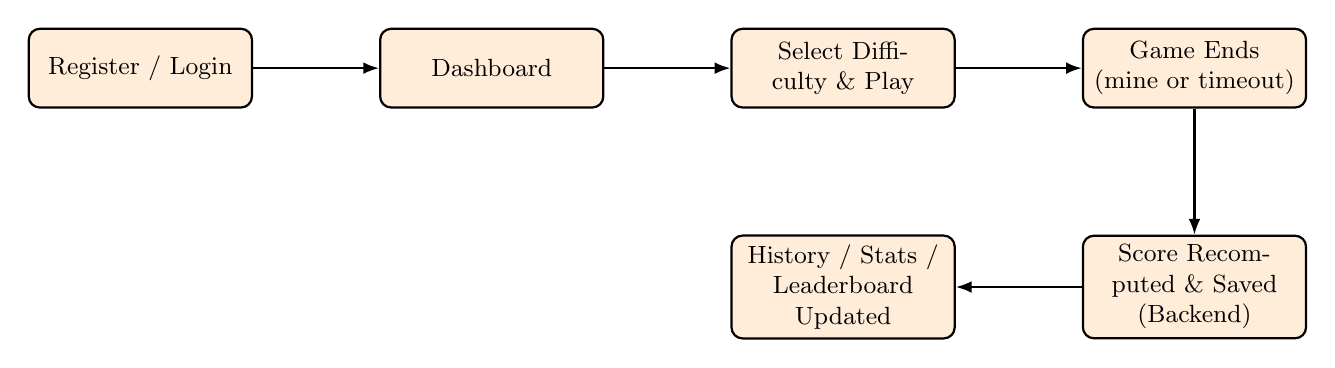
\begin{tikzpicture}[node distance=1.6cm, every node/.style={font=\small}]
        \tikzstyle{block} = [rectangle, rounded corners, draw=black, thick,
            fill=orange!15, text width=2.6cm, align=center, minimum height=1cm]
        \tikzstyle{arrow} = [-{Latex[length=2mm]}, thick]

        \node (login) [block] {Register / Login};
        \node (dash) [block, right=of login] {Dashboard};
        \node (play) [block, right=of dash] {Select Difficulty \& Play};
        \node (end) [block, right=of play] {Game Ends \\ (mine or timeout)};
        \node (save) [block, below=of end] {Score Recomputed \& Saved (Backend)};
        \node (views) [block, left=of save] {History / Stats / Leaderboard Updated};

        \draw [arrow] (login) -- (dash);
        \draw [arrow] (dash) -- (play);
        \draw [arrow] (play) -- (end);
        \draw [arrow] (end) -- (save);
        \draw [arrow] (save) -- (views);
    \end{tikzpicture}
    \caption{High-level player workflow.}
    \label{fig:user-flow}
\end{figure}

\section{Main Modules}
The application is organized into the following functional areas, described
in detail in later chapters:
\begin{itemize}[nosep]
    \item \textbf{Authentication Module} -- registration, login, and logout
    endpoints backed by PHP sessions (\texttt{register.php},
    \texttt{login.php}, \texttt{logout.php}).
    \item \textbf{Game Engine Module} -- the pure functional board logic in
    \texttt{minesweeper.js} and the stateful \texttt{useMinesweeper} hook
    that drives it.
    \item \textbf{Score Persistence Module} -- the \texttt{save-score.php}
    endpoint, which validates and recomputes a submitted result before
    writing it to the \texttt{game\_results} table.
    \item \textbf{Statistics and History Module} -- the
    \texttt{leaderboard.php}, \texttt{history.php}, and \texttt{stats.php}
    endpoints and their corresponding React pages.
\end{itemize}

\section{Screenshots}
Figures~\ref{fig:login-page} and~\ref{fig:register-page} show the
authentication screens; Figure~\ref{fig:dashboard-page} shows the
authenticated dashboard.

\begin{figure}[h]
    \centering
    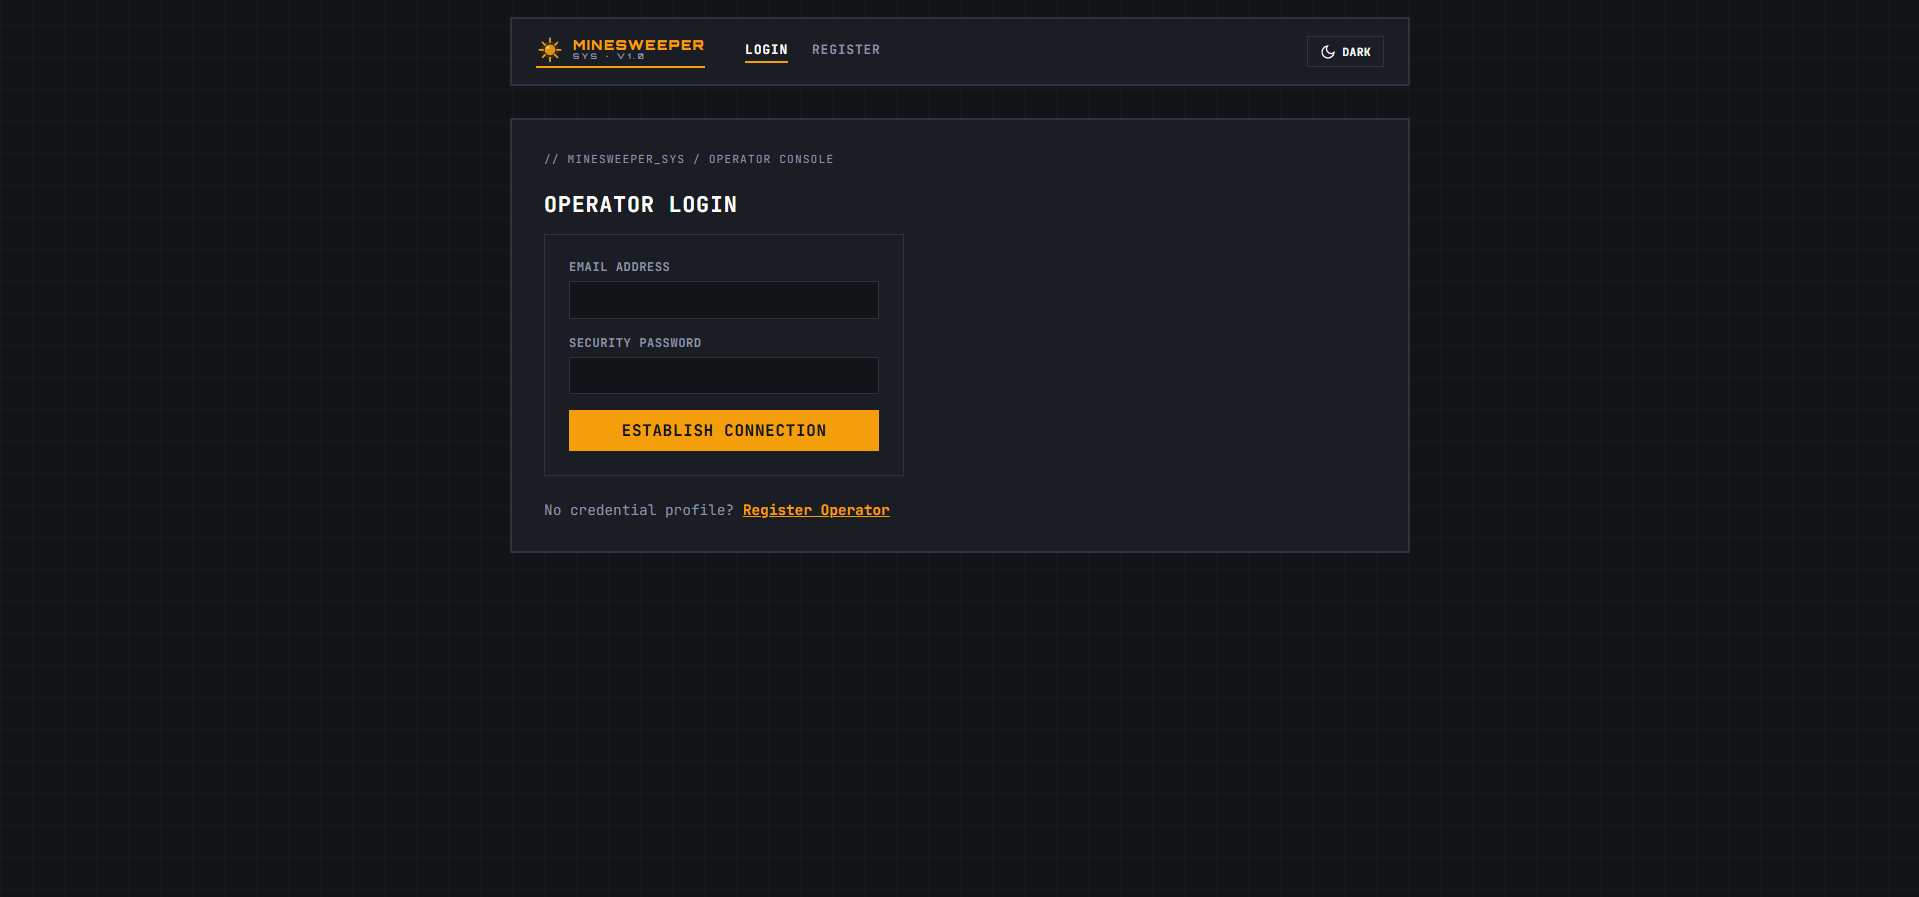
\includegraphics[width=0.8\textwidth]{figures/fig_login.png}
    \caption{Operator login page.}
    \label{fig:login-page}
\end{figure}

\begin{figure}[h]
    \centering
    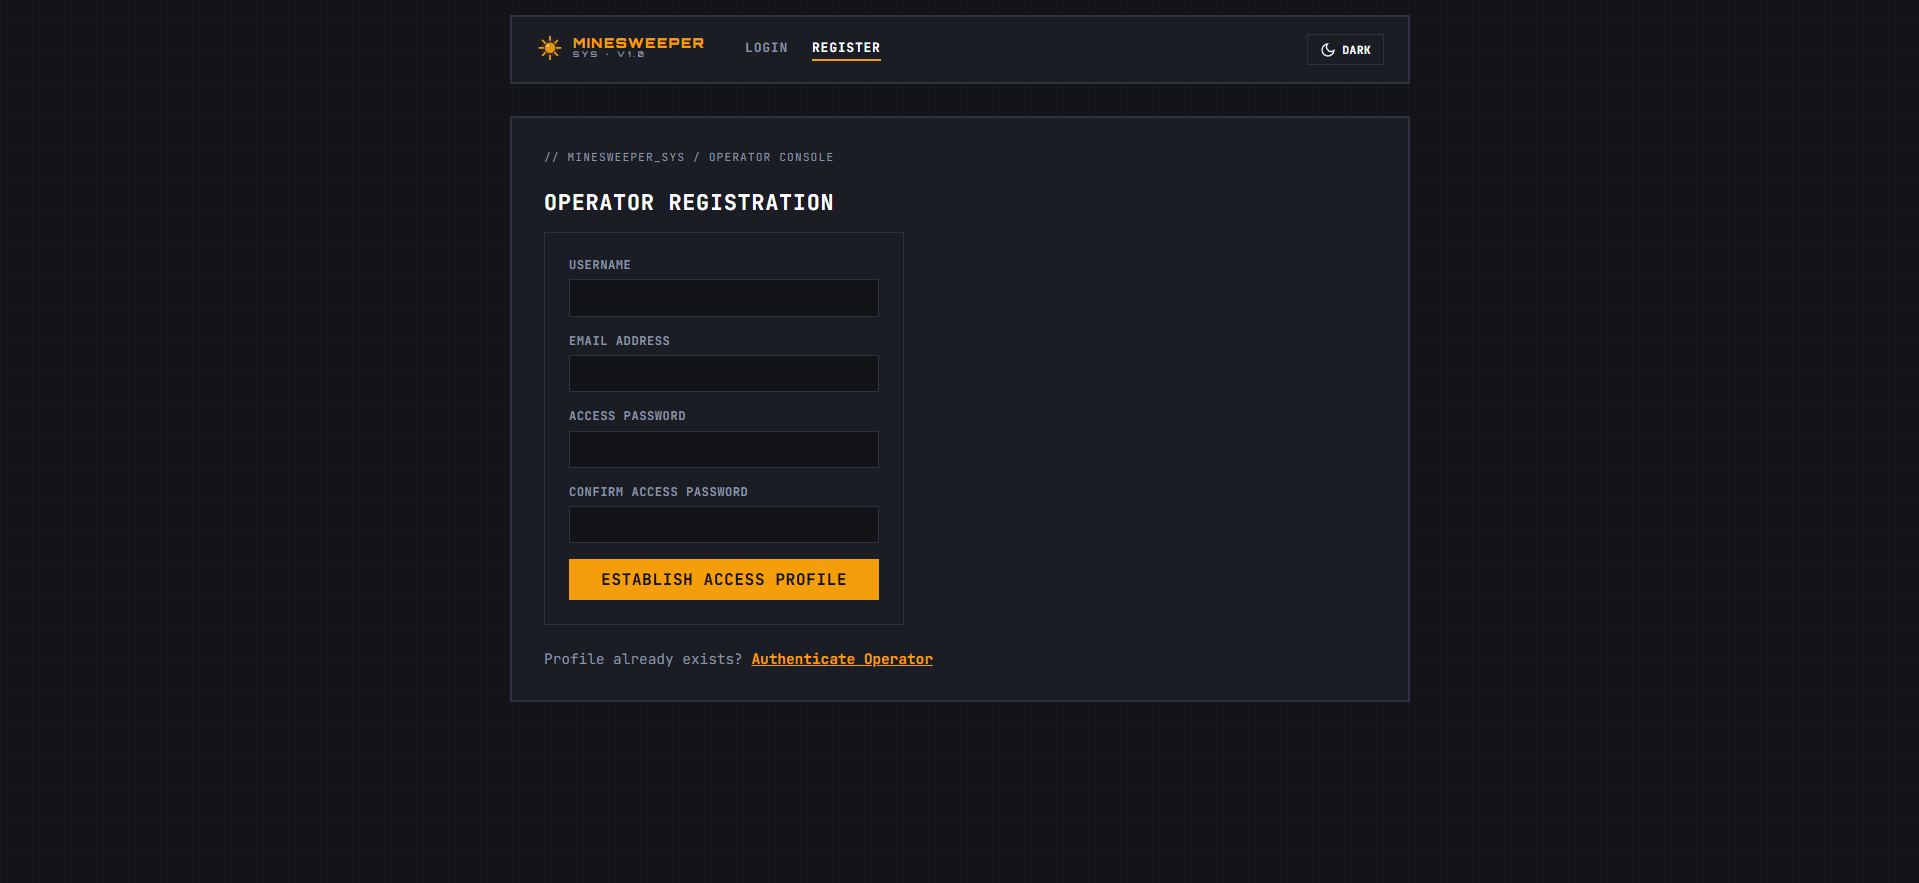
\includegraphics[width=0.8\textwidth]{figures/fig_register.png}
    \caption{Operator registration page.}
    \label{fig:register-page}
\end{figure}

\begin{figure}[h]
    \centering
    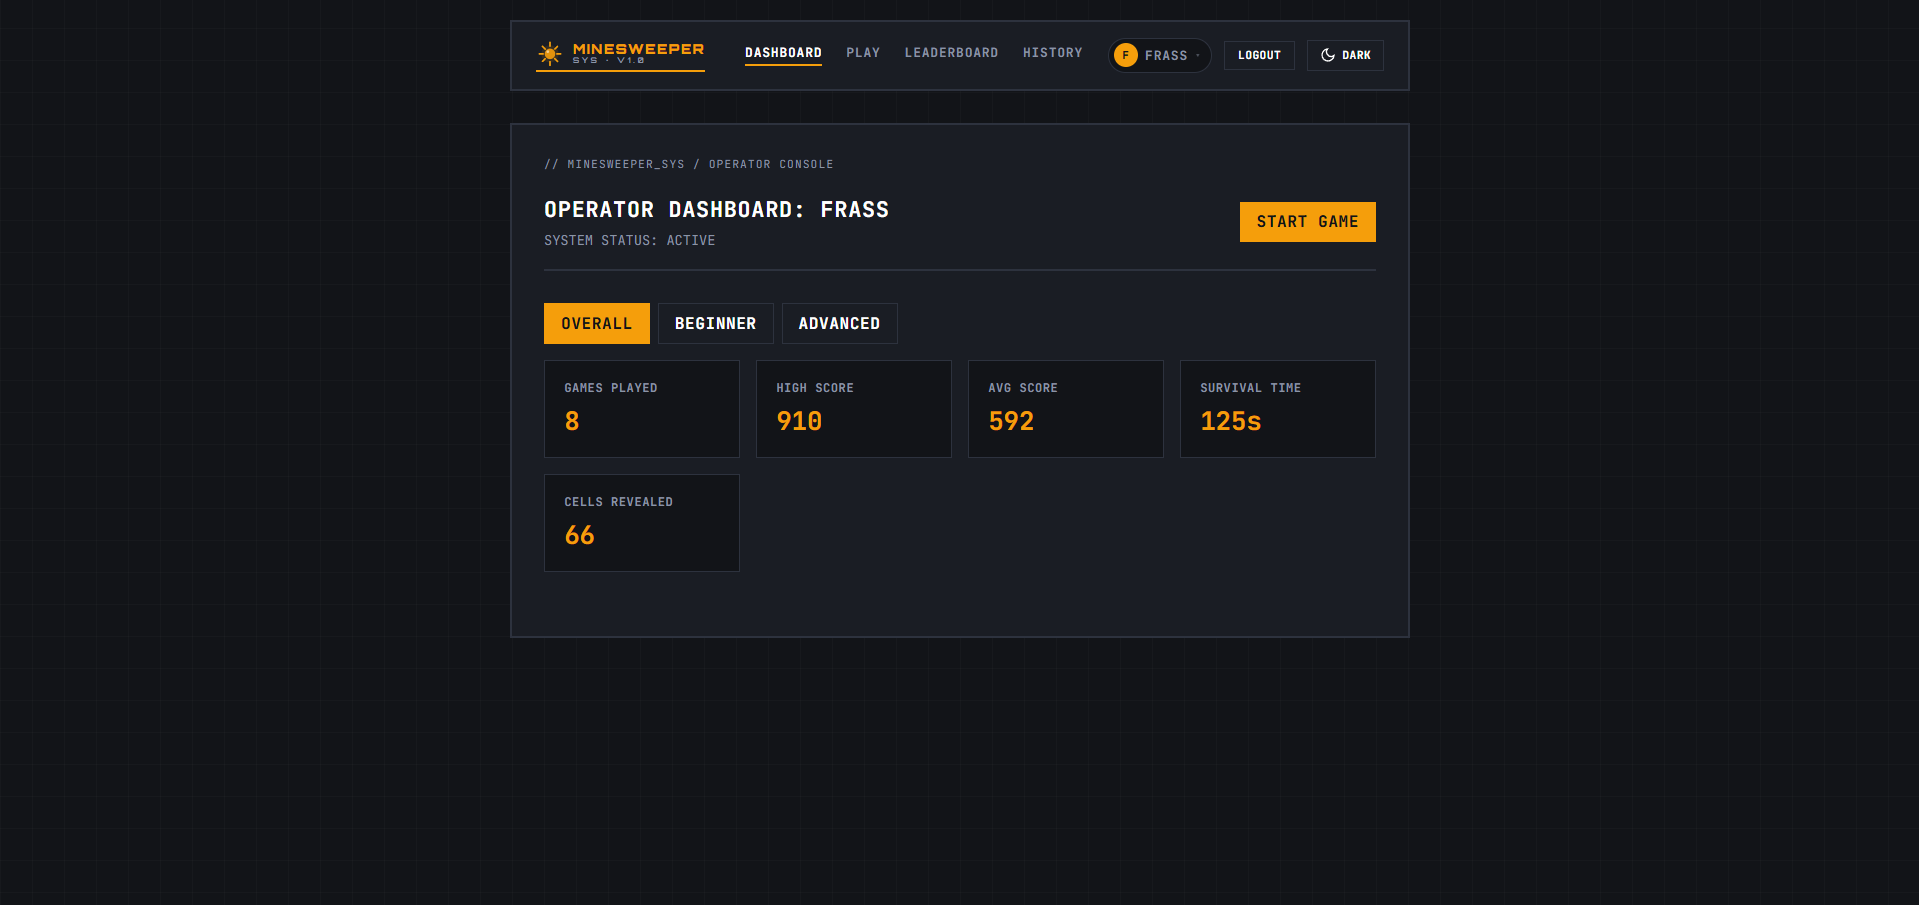
\includegraphics[width=0.8\textwidth]{figures/fig_dashboard_dark.png}
    \caption{Player dashboard showing combat statistics and quick-access links.}
    \label{fig:dashboard-page}
\end{figure}

\chapter{Requirements Analysis}
\label{ch:requirements}

\section{Functional Requirements}
The functional requirements below are derived directly from the behaviour
implemented in the source code.

\begin{enumerate}[nosep]
    \item The system shall allow a new user to register with a username
    (3--50 characters), an email address, and a password of at least 6
    characters, confirmed twice.
    \item The system shall reject registration when the supplied email is
    not a valid email address, or when the username or email is already in
    use.
    \item The system shall hash passwords with \texttt{password\_hash()}
    before storing them, and never store plaintext passwords.
    \item The system shall allow a registered user to log in with their
    email and password, verified with \texttt{password\_verify()}, and shall
    regenerate the session ID on successful login.
    \item The system shall allow a logged-in user to log out, which clears
    and destroys the server-side session.
    \item The system shall allow a logged-in user to start a game at one of
    two difficulties: Beginner ($9\times9$, 10 mines) or Advanced
    ($16\times16$, 40 mines).
    \item The system shall guarantee that the first cell revealed by the
    player, and all of its immediate neighbours, never contain a mine.
    \item The system shall reveal a cascade of adjacent zero-value cells
    automatically when a zero-adjacency cell is revealed (flood reveal).
    \item The system shall allow the player to flag and unflag unrevealed
    cells, up to the total mine count for the active difficulty.
    \item The system shall allow the player to chord on a revealed numbered
    cell when the number of adjacent flags equals its adjacent mine count,
    automatically revealing the remaining unflagged neighbours.
    \item The system shall allow the player up to 3 hints per game, each
    highlighting a random unrevealed, non-mine cell for 3 seconds.
    \item The system shall grant the player exactly one shield per game,
    which, once activated, prevents the next mine reveal from ending the
    game.
    \item The system shall end the game when the player reveals a mine
    (without an active shield) or when the 120-second timer reaches zero,
    and shall reveal all mines at that point.
    \item The system shall automatically submit the completed game's
    metrics (difficulty, time taken, cells revealed, hints used) to the
    backend once, and shall not re-submit the same completed game.
    \item The system shall recompute the score on the server from the
    submitted metrics rather than accept a client-supplied score, and shall
    reject metric values that fall outside the valid range for the given
    difficulty.
    \item The system shall reject a duplicate submission of the same result
    signature (user, difficulty, time, cells, hints) received within 10
    seconds of the previous one.
    \item The system shall display, for a logged-in user: personal
    statistics (games played, high score, average score, longest survival,
    most cells revealed), a history of up to 200 past games, and a global
    top-10 leaderboard, each filterable by difficulty.
\end{enumerate}

\section{Non-Functional Requirements}
\begin{itemize}[nosep]
    \item \textbf{Security} -- passwords must never be stored in plaintext;
    all SQL queries that include user input must use PDO prepared
    statements; session cookies must be HTTP-only; cross-origin requests
    must be restricted to an explicit allow-list of origins.
    \item \textbf{Data Integrity} -- the \texttt{users} table must guarantee
    unique usernames and unique email addresses; every stored game result
    must be linked to a valid user via a foreign key.
    \item \textbf{Usability} -- the interface should allow a player to start
    a game, understand their remaining time, mines, flags, and score, and
    review a completed game's outcome, without external instructions.
    \item \textbf{Maintainability} -- difficulty parameters (grid size, mine
    count) should be defined in a single, centralized configuration object
    on the frontend rather than duplicated across components.
\end{itemize}

\section{User Requirements}
A player needs an account, a way to start and play a timed game at a chosen
difficulty, visible feedback on their current score and remaining time and
mines, a way to review their past results, and a way to compare their best
scores against other players.

\section{Requirements Traceability}
Table~\ref{tab:req-trace} maps a representative subset of the functional
requirements above to the test cases used to validate them in
Chapter~\ref{ch:testing}.

\begin{table}[h]
\centering
\caption{Representative requirements-to-test-case mapping.}
\label{tab:req-trace}
\begin{tabular}{@{}p{2.2cm}p{9cm}p{1.5cm}@{}}
\toprule
\textbf{Req.\ \#} & \textbf{Requirement} & \textbf{Test ID} \\
\midrule
FR-3  & Password hashing on registration & T-2 \\
FR-7  & First-click safety & T-4 \\
FR-8  & Flood-fill cascade & T-5 \\
FR-10 & Chording precondition & T-6 \\
FR-12 & Shield blocks next mine reveal & T-7 \\
FR-15 & Server-side score recomputation & T-9 \\
FR-16 & Duplicate-submission rejection & T-10 \\
\bottomrule
\end{tabular}
\end{table}

\chapter{Game Design and Algorithms}
\label{ch:game-design}

This chapter describes the core Minesweeper game engine, implemented as a
set of pure functions in \texttt{frontend/src/utils/minesweeper.js} and
driven by the stateful hook \texttt{useMinesweeper.js}. Because the game
engine is the technical core of this project, it is treated here as a
dedicated chapter rather than as a subsection of the general implementation
chapter.

\section{Board Representation}
The board is represented as a two-dimensional array of cell objects. Each
cell has four fields:
\begin{itemize}[nosep]
    \item \texttt{isMine} -- whether the cell contains a mine.
    \item \texttt{isRevealed} -- whether the cell has been uncovered.
    \item \texttt{isFlagged} -- whether the player has marked the cell.
    \item \texttt{adjacentMines} -- the count of mines among the cell's up
    to 8 neighbours.
\end{itemize}
\texttt{createEmptyBoard} builds this grid with every cell initialised to
safe, unrevealed, and unflagged, before any mines are placed.

\section{Difficulty Configuration}
Two difficulties are defined in a single configuration object,
\texttt{DIFFICULTIES}, shown in Table~\ref{tab:difficulties}. Centralising
these values avoids duplicating grid dimensions across components.

\begin{table}[h]
\centering
\caption{Supported difficulty configurations.}
\label{tab:difficulties}
\begin{tabular}{@{}lccc@{}}
\toprule
\textbf{Difficulty} & \textbf{Grid} & \textbf{Mines} & \textbf{Safe Cells} \\
\midrule
Beginner & $9 \times 9$   & 10 & 71 \\
Advanced & $16 \times 16$ & 40 & 216 \\
\bottomrule
\end{tabular}
\end{table}

\section{First-Click Safety}
\label{sec:first-click}
Mines are not placed when the board is created; they are placed only in
response to the player's first reveal, via \texttt{placeMines(board,
mineCount, safeRow, safeCol)}. The function first builds a set containing
the clicked cell and all of its neighbours (up to 8 cells), marking them as
off-limits to mine placement. It then builds a list of every remaining
candidate cell, shuffles it with a Fisher--Yates shuffle, and takes the
first \texttt{mineCount} cells from the shuffled list as mine positions.
Finally, it computes \texttt{adjacentMines} for every non-mine cell by
counting mines among its neighbours. This guarantees that a player's first
click, and the small neighbourhood around it, can never immediately end the
game.

\begin{lstlisting}[language=JavaScript, caption={Simplified first-click safety and mine placement (\texttt{minesweeper.js}).}, label={lst:place-mines}]
export function placeMines(board, mineCount, safeRow, safeCol) {
  const safeCells = new Set([`${safeRow},${safeCol}`]);
  getNeighbors(board, safeRow, safeCol).forEach((cell) => {
    safeCells.add(`${cell.row},${cell.col}`);
  });

  const candidates = [];
  for (let row = 0; row < board.length; row++) {
    for (let col = 0; col < board[0].length; col++) {
      if (!safeCells.has(`${row},${col}`)) candidates.push([row, col]);
    }
  }

  // Fisher-Yates shuffle
  for (let i = candidates.length - 1; i > 0; i--) {
    const j = Math.floor(Math.random() * (i + 1));
    [candidates[i], candidates[j]] = [candidates[j], candidates[i]];
  }

  const mineCells = candidates.slice(0, mineCount);
  // ... mark mineCells as isMine = true, then compute adjacentMines
}
\end{lstlisting}

\section{Flood-Fill Reveal Algorithm}
\label{sec:flood-fill}
When a cell with \texttt{adjacentMines === 0} is revealed, all of its
neighbours are safe to reveal automatically, and this cascades outward until
every reachable zero-adjacency region and its numbered border has been
uncovered. This is implemented in \texttt{revealCell(board, row, col)} using
an explicit stack rather than recursion, which avoids call-stack depth
concerns on larger boards such as the $16\times16$ Advanced grid. Each
iteration pops a coordinate, skips it if already revealed or flagged,
reveals it, and -- if it has zero adjacent mines and is not a mine -- pushes
its unrevealed, unflagged neighbours onto the stack for processing.

\begin{lstlisting}[language=JavaScript, caption={Iterative flood-fill reveal (\texttt{minesweeper.js}).}, label={lst:flood-fill}]
export function revealCell(board, row, col) {
  const newBoard = board.map((r) => r.map((cell) => ({ ...cell })));
  const stack = [[row, col]];

  while (stack.length > 0) {
    const [r, c] = stack.pop();
    const cell = newBoard[r][c];
    if (cell.isRevealed || cell.isFlagged) continue;
    cell.isRevealed = true;

    if (cell.adjacentMines === 0 && !cell.isMine) {
      getNeighbors(newBoard, r, c).forEach((neighbor) => {
        if (!neighbor.isRevealed && !neighbor.isFlagged) {
          stack.push([neighbor.row, neighbor.col]);
        }
      });
    }
  }
  return newBoard;
}
\end{lstlisting}

Figure~\ref{fig:flood-fill-example} illustrates a worked example: revealing
a single zero-adjacency cell cascades outward until it reaches cells with a
non-zero mine count, which are revealed but do not propagate further.

\begin{figure}[h]
\centering
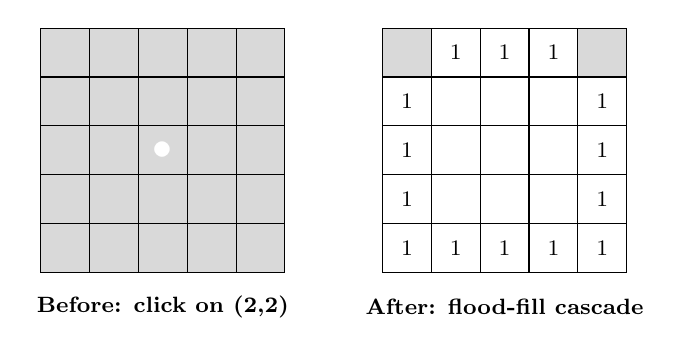
\begin{tikzpicture}[scale=0.62, every node/.style={font=\footnotesize}]
  % Before grid
  \begin{scope}
    \foreach \x in {0,...,4} {
      \foreach \y in {0,...,4} {
        \draw[fill=gray!30] (\x,\y) rectangle ++(1,1);
      }
    }
    \node at (2.5,-0.7) {\textbf{Before: click on (2,2)}};
    \node at (2.5,2.5) {\textcolor{white}{\Large $\bullet$}};
  \end{scope}
  % After grid
  \begin{scope}[xshift=7cm]
    \foreach \x in {0,...,4} {
      \foreach \y in {0,...,4} {
        \draw[fill=gray!30] (\x,\y) rectangle ++(1,1);
      }
    }
    % revealed cascade (zeros) - center cross region
    \foreach \x/\y in {1/1,2/1,3/1,1/2,2/2,3/2,1/3,2/3,3/3} {
      \draw[fill=white] (\x,\y) rectangle ++(1,1);
    }
    % bordering numbered cells: draw the white fills FIRST, then the
    % number labels on top, so the labels stay visible
    \draw[fill=white] (0,0) rectangle ++(1,1);
    \draw[fill=white] (0,1) rectangle ++(1,1);
    \draw[fill=white] (0,2) rectangle ++(1,1);
    \draw[fill=white] (0,3) rectangle ++(1,1);
    \draw[fill=white] (4,0) rectangle ++(1,1);
    \draw[fill=white] (4,1) rectangle ++(1,1);
    \draw[fill=white] (4,2) rectangle ++(1,1);
    \draw[fill=white] (4,3) rectangle ++(1,1);
    \draw[fill=white] (1,0) rectangle ++(1,1);
    \draw[fill=white] (2,0) rectangle ++(1,1);
    \draw[fill=white] (3,0) rectangle ++(1,1);
    \draw[fill=white] (1,4) rectangle ++(1,1);
    \draw[fill=white] (2,4) rectangle ++(1,1);
    \draw[fill=white] (3,4) rectangle ++(1,1);
    \node at (0.5,0.5) {1};
    \node at (0.5,1.5) {1};
    \node at (0.5,2.5) {1};
    \node at (0.5,3.5) {1};
    \node at (4.5,0.5) {1};
    \node at (4.5,1.5) {1};
    \node at (4.5,2.5) {1};
    \node at (4.5,3.5) {1};
    \node at (1.5,0.5) {1};
    \node at (2.5,0.5) {1};
    \node at (3.5,0.5) {1};
    \node at (1.5,4.5) {1};
    \node at (2.5,4.5) {1};
    \node at (3.5,4.5) {1};
    \node at (2.5,-0.7) {\textbf{After: flood-fill cascade}};
  \end{scope}
\end{tikzpicture}
\caption{Worked example of the flood-fill reveal: clicking a zero-adjacency
cell cascades to reveal the surrounding zero region and its numbered
border, while unrelated cells remain hidden.}
\label{fig:flood-fill-example}
\end{figure}

\section{Flagging}
\texttt{toggleFlag(board, row, col, mineCount)} toggles a cell's flag state.
A revealed cell cannot be flagged. A new flag is only placed if the current
number of flags on the board (\texttt{countFlags}) is below the mine count
for the active difficulty, preventing the flag counter from going negative
in the UI.

\section{Chording}
\label{sec:chording}
Chording lets the player reveal all unflagged neighbours of an
already-revealed numbered cell in one action, once the surrounding flags
match its number. \texttt{chordCell(board, row, col)} first checks that the
target cell is revealed, has a non-zero \texttt{adjacentMines} value, and is
not itself a mine. It then counts flagged neighbours; if that count does not
equal \texttt{adjacentMines}, the board is returned unchanged. Otherwise,
every unflagged, unrevealed neighbour is revealed via \texttt{revealCell}
(triggering flood-fill where applicable). If a chord reveals a mine -- i.e.\
the player mis-flagged -- the calling code in \texttt{useMinesweeper}
detects a revealed mine cell in the resulting board and ends the game.

\begin{lstlisting}[language=JavaScript, caption={Chording logic (\texttt{minesweeper.js}).}, label={lst:chord}]
export function chordCell(board, row, col) {
  const cell = board[row][col];
  if (!cell.isRevealed || cell.adjacentMines === 0 || cell.isMine) return board;

  const neighbors = getNeighbors(board, row, col);
  const adjacentFlagCount = neighbors.filter((n) => n.isFlagged).length;
  if (adjacentFlagCount !== cell.adjacentMines) return board;

  let workingBoard = board;
  neighbors
    .filter((n) => !n.isFlagged && !n.isRevealed)
    .forEach((n) => { workingBoard = revealCell(workingBoard, n.row, n.col); });
  return workingBoard;
}
\end{lstlisting}

\section{Hint System}
\texttt{findHintCell(board)} collects every cell that is not a mine, not
revealed, and not flagged, and returns one at random. The calling hook
records the hint usage (capped at \texttt{MAX\_HINTS = 3}), stores the
returned coordinates as the currently highlighted \texttt{hintCell}, and
clears the highlight after \texttt{HINT\_HIGHLIGHT\_MS = 3000} milliseconds
via a timeout. Each hint used subtracts \texttt{HINT\_COST = 50} points from
the eventual score (Section~\ref{sec:scoring}).

\section{Shield Ability}
Each game grants the player exactly one shield, tracked as a three-state
value: \texttt{available}, \texttt{active}, and \texttt{used}. Activating
the shield (\texttt{activateShield}) is only permitted while it is
\texttt{available}. While \texttt{active}, the next time the player reveals
a mine, \texttt{revealCellAt} sets the shield to \texttt{used} and returns
without ending the game or revealing the mine, letting play continue.
Figure~\ref{fig:shield-state} shows the shield's state machine. Note that
because mines are placed only on the first click
(Section~\ref{sec:first-click}), an active shield can, in principle, be
consumed by the very first reveal if that reveal happens to land on a
mine-designated cell outside the guaranteed-safe neighbourhood -- though in
practice first-click safety makes this impossible for the first click
itself, and the shield instead protects the player's first mine encounter
on any later click.

\begin{figure}[htbp]
\centering
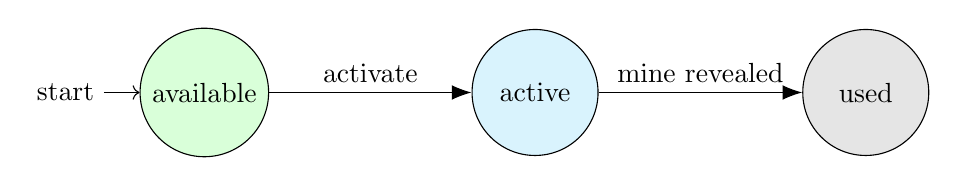
\begin{tikzpicture}[node distance=4.2cm, on grid, auto,
    every state/.style={minimum size=1.6cm}]
  \node[state, initial, fill=green!15] (avail) {available};
  \node[state, right=of avail, fill=cyan!15] (active) {active};
  \node[state, right=of active, fill=gray!20] (used) {used};

  \path[-{Latex[length=2.5mm]}]
    (avail) edge node[above, text width=2.2cm, align=center] {activate} (active)
    (active) edge node[above, text width=2.6cm, align=center] {mine revealed} (used);
\end{tikzpicture}
\caption{Shield ability state machine.}
\label{fig:shield-state}
\end{figure}

\section{Game State Machine}
The overall game progresses through three states, tracked as
\texttt{gameStatus} in \texttt{useMinesweeper}: \texttt{ready} (board
created but mines not yet placed), \texttt{playing} (first click made,
timer running), and \texttt{lost} (a mine was revealed without an active
shield, or the timer reached zero). There is deliberately no
\texttt{won}/\texttt{completed-board} state.

\begin{figure}[htbp]
\centering
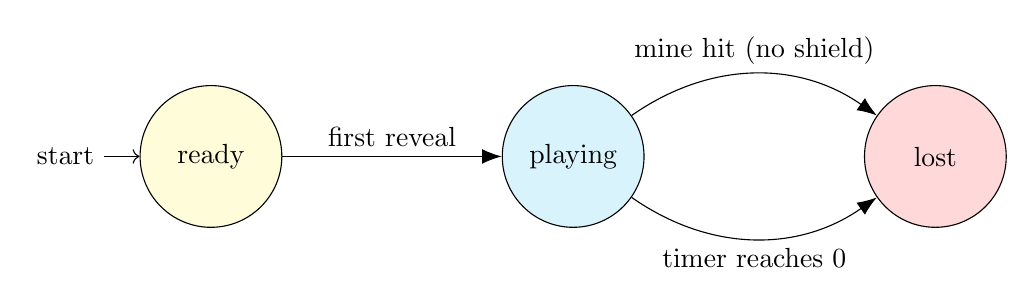
\begin{tikzpicture}[node distance=4.6cm, on grid, auto,
    every state/.style={minimum size=1.8cm}]
  \node[state, initial, fill=yellow!15] (ready) {ready};
  \node[state, right=of ready, fill=cyan!15] (playing) {playing};
  \node[state, right=of playing, fill=red!15] (lost) {lost};

  \path[-{Latex[length=2.5mm]}]
    (ready) edge node[above, text width=2.4cm, align=center] {first reveal} (playing)
    (playing) edge[bend left=35] node[above, text width=3.2cm, align=center] {mine hit (no shield)} (lost)
    (playing) edge[bend right=35] node[below, text width=2.6cm, align=center] {timer reaches 0} (lost);
\end{tikzpicture}
\caption{Game status state machine. There is no explicit ``won'' state; the
game is a timed survival mode.}
\label{fig:game-state}
\end{figure}

\section{Survival Mode and the Absence of a Win Condition}
Every game begins with a fixed countdown of \texttt{TIME\_LIMIT\_SECONDS =
120}. The game does not end when all safe cells are revealed; the player may
continue revealing cells (subject to normal Minesweeper deduction) until
either a mine is hit or the timer expires. This design choice is reflected
in the database schema (Chapter~\ref{ch:database}), which stores
\texttt{cells\_revealed} and \texttt{time\_taken} but has no
\texttt{result}/win-loss column -- an explicit migration
(\texttt{migration-remove-win-condition.sql}) removed a previous
\texttt{result} column when survival mode was adopted.

\section{Scoring Formula}
\label{sec:scoring}
The score for a completed game is:
\[
\text{score} = \max\bigl(0,\; (\text{cellsRevealed} \times 10) +
(\text{timeElapsed} \times 0) - (\text{hintsUsed} \times 50)\bigr)
\]
\texttt{POINTS\_PER\_SECOND} is deliberately set to \texttt{0}. Although the
constant exists in the formula, it is defined as zero specifically to
prevent a player from inflating their score simply by surviving passively
(e.g.\ letting the timer run without revealing cells); the score is driven
entirely by the number of safe cells actually revealed, less a fixed penalty
per hint used. The same formula is evaluated twice: once on the client for
immediate UI feedback (\texttt{calculateScore} in \texttt{minesweeper.js}),
and independently on the server when the result is saved
(Section~\ref{sec:score-validation}), so that the value shown to the player
during play is never the value actually trusted for the leaderboard.

\begin{lstlisting}[language=JavaScript, caption={Client-side score formula (\texttt{minesweeper.js}).}, label={lst:score}]
export const POINTS_PER_CELL = 10;
export const POINTS_PER_SECOND = 0;
export const HINT_COST = 50;

export function calculateScore(cellsRevealed, timeElapsed, hintsUsed) {
  const rawScore = cellsRevealed * POINTS_PER_CELL
                  + timeElapsed * POINTS_PER_SECOND
                  - hintsUsed * HINT_COST;
  return Math.max(0, rawScore);
}
\end{lstlisting}

\section{Decision Flow of a Cell Reveal}
Figure~\ref{fig:reveal-flow} summarises the decision logic executed each
time the player clicks a cell, as implemented in \texttt{revealCellAt}
within \texttt{useMinesweeper.js}.

\begin{figure}[p]
\centering
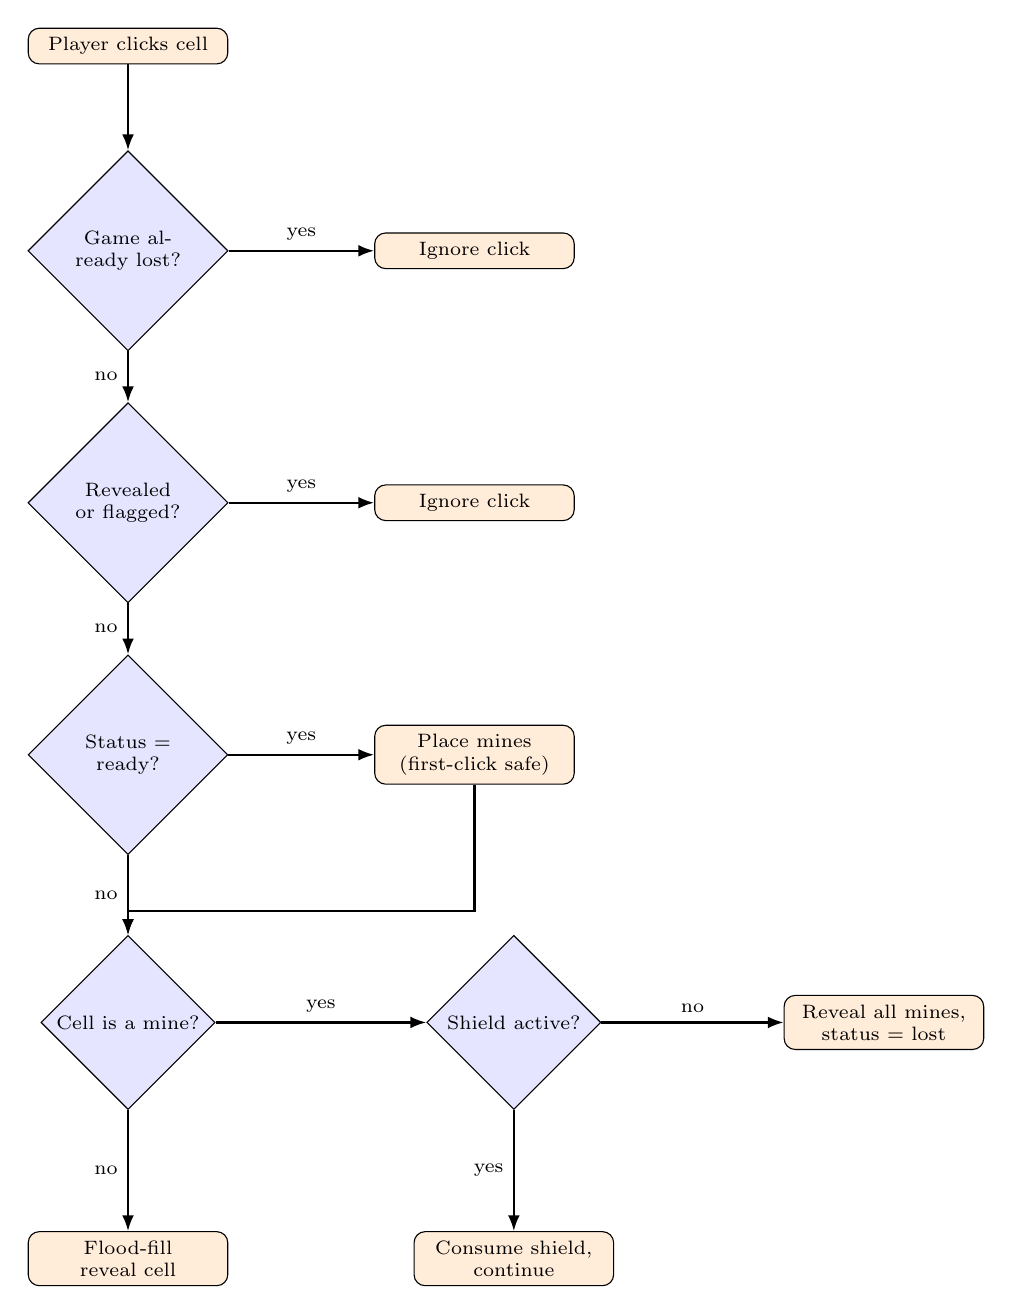
\begin{tikzpicture}[every node/.style={font=\scriptsize}]
  \tikzstyle{decision} = [diamond, draw, fill=blue!10, text width=1.9cm,
      align=center, inner sep=1pt]
  \tikzstyle{action} = [rectangle, draw, fill=orange!15, text width=2.3cm,
      align=center, rounded corners]
  \tikzstyle{arrow} = [-{Latex[length=2mm]}, thick]

  % Column x-positions: A = main spine, B = first branch column,
  % C = second branch column. Rows are spaced generously (3.1cm) so that
  % the wide diamond shapes never touch their neighbours.
  \node (start)      [action]              at (0,0)      {Player clicks cell};
  \node (lostcheck)  [decision]            at (0,-2.6)    {Game already lost?};
  \node (stop1)      [action]              at (4.4,-2.6)  {Ignore click};
  \node (statecheck) [decision]            at (0,-5.8)    {Revealed or flagged?};
  \node (stop2)      [action]              at (4.4,-5.8)  {Ignore click};
  \node (readycheck) [decision]            at (0,-9.0)    {Status = ready?};
  \node (place)      [action]              at (4.4,-9.0)  {Place mines (first-click safe)};
  \node (minecheck)  [decision]            at (0,-12.4)   {Cell is a mine?};
  \node (shieldcheck)[decision]            at (4.9,-12.4) {Shield active?};
  \node (lose)       [action]              at (9.6,-12.4) {Reveal all mines, status = lost};
  \node (reveal)     [action]              at (0,-15.4)   {Flood-fill reveal cell};
  \node (consume)    [action]              at (4.9,-15.4) {Consume shield, continue};

  \draw[arrow] (start) -- (lostcheck);
  \draw[arrow] (lostcheck) -- node[above] {yes} (stop1);
  \draw[arrow] (lostcheck) -- node[left] {no} (statecheck);
  \draw[arrow] (statecheck) -- node[above] {yes} (stop2);
  \draw[arrow] (statecheck) -- node[left] {no} (readycheck);
  \draw[arrow] (readycheck) -- node[above] {yes} (place);
  \draw[arrow] (readycheck) -- node[left] {no} (minecheck);
  % Feedback path from "place mines" back into the main spine: dips down
  % in the empty gap between column A and column B, well clear of the
  % "Shield active?" diamond, before entering minecheck from the top.
  \draw[arrow] (place.south) -- ++(0,-1.6) -| (minecheck.north);
  \draw[arrow] (minecheck) -- node[above] {yes} (shieldcheck);
  \draw[arrow] (minecheck) -- node[left] {no} (reveal);
  \draw[arrow] (shieldcheck) -- node[above] {no} (lose);
  \draw[arrow] (shieldcheck) -- node[left] {yes} (consume);
\end{tikzpicture}
\caption{Decision flow for handling a cell reveal in \texttt{revealCellAt}.}
\label{fig:reveal-flow}
\end{figure}

\chapter{System Architecture and Software Design}
\label{ch:architecture}

\section{Overall Architecture}
The application follows a three-tier architecture, but unlike a classic
server-rendered PHP application, the frontend is a React single-page
application that communicates with the backend purely through a JSON API,
rather than through full-page navigations. Figure~\ref{fig:architecture}
shows the overall structure.

\begin{figure}[h]
\centering
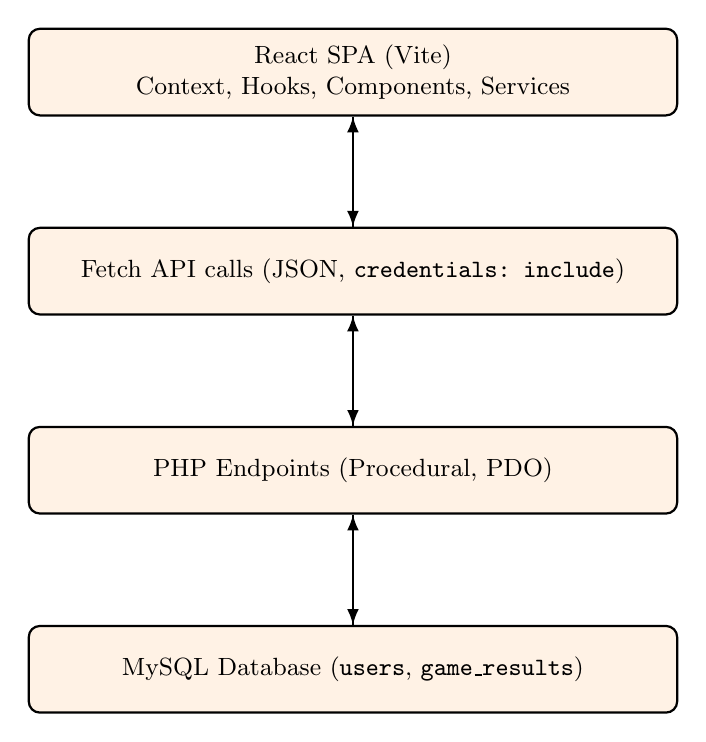
\begin{tikzpicture}[node distance=1.4cm, every node/.style={font=\small}]
    \tikzstyle{tier} = [rectangle, draw=black, thick, rounded corners,
        fill=orange!10, text width=8cm, align=center, minimum height=1.1cm]
    \node (client) [tier] {React SPA (Vite) \\ Context, Hooks, Components, Services};
    \node (api) [tier, below=of client] {Fetch API calls (JSON, \texttt{credentials: include})};
    \node (backend) [tier, below=of api] {PHP Endpoints (Procedural, PDO)};
    \node (db) [tier, below=of backend] {MySQL Database (\texttt{users}, \texttt{game\_results})};

    \draw [-{Latex[length=2mm]}, thick] (client) -- (api);
    \draw [-{Latex[length=2mm]}, thick] (api) -- (backend);
    \draw [-{Latex[length=2mm]}, thick] (backend) -- (db);
    \draw [-{Latex[length=2mm]}, thick] (db) -- (backend);
    \draw [-{Latex[length=2mm]}, thick] (backend) -- (api);
    \draw [-{Latex[length=2mm]}, thick] (api) -- (client);
\end{tikzpicture}
\caption{Overall three-tier architecture of the application.}
\label{fig:architecture}
\end{figure}

\section{Frontend Architecture}
The frontend is organised into four layers:
\begin{itemize}[nosep]
    \item \textbf{Context providers} -- \texttt{AuthContext} holds the
    current user and authentication status; \texttt{ThemeContext} holds the
    light/dark theme preference; a \texttt{ToastContext} manages transient
    notification messages.
    \item \textbf{Custom hooks} -- \texttt{useMinesweeper} is the central
    state machine for a single game session, wrapping the pure functions
    from Chapter~\ref{ch:game-design} with React state and effects (the
    countdown timer, hint highlight timeout, and automatic score
    submission).
    \item \textbf{Components / Pages} -- page-level components
    (Login, Register, Dashboard, Game, Leaderboard, History) composed from
    smaller presentational components (the board grid, a cell, the
    stats cards).
    \item \textbf{Services} -- \texttt{api.js} wraps the browser
    \texttt{fetch} API with a consistent JSON request/response contract;
    \texttt{authService.js} and \texttt{gameService.js} expose
    typed functions (e.g.\ \texttt{login}, \texttt{register},
    \texttt{saveScore}, \texttt{getLeaderboard}) built on top of it.
\end{itemize}

\begin{figure}[h]
\centering
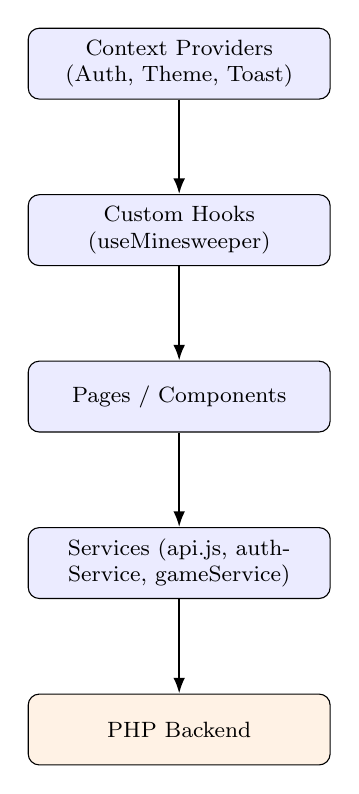
\begin{tikzpicture}[node distance=1.2cm, every node/.style={font=\footnotesize}]
    \tikzstyle{box} = [rectangle, draw=black, rounded corners, fill=blue!8,
        text width=3.6cm, align=center, minimum height=0.9cm]
    \node (ctx) [box] {Context Providers \\ (Auth, Theme, Toast)};
    \node (hooks) [box, below=of ctx] {Custom Hooks \\ (useMinesweeper)};
    \node (comp) [box, below=of hooks] {Pages / Components};
    \node (svc) [box, below=of comp] {Services (api.js, authService, gameService)};
    \node (backend) [box, below=of svc, fill=orange!10] {PHP Backend};

    \draw [-{Latex[length=2mm]}, thick] (ctx) -- (hooks);
    \draw [-{Latex[length=2mm]}, thick] (hooks) -- (comp);
    \draw [-{Latex[length=2mm]}, thick] (comp) -- (svc);
    \draw [-{Latex[length=2mm]}, thick] (svc) -- (backend);
\end{tikzpicture}
\caption{Frontend layered data flow.}
\label{fig:frontend-layers}
\end{figure}

\section{Backend Architecture}
The backend is written in procedural PHP, organised as one script per
endpoint (e.g.\ \texttt{register.php}, \texttt{login.php},
\texttt{save-score.php}, \texttt{leaderboard.php}, \texttt{history.php},
\texttt{stats.php}), plus shared includes for the database connection and
session/authentication helpers. Every protected endpoint begins by calling a
shared \texttt{require\_login()} helper, which checks the PHP session for a
logged-in user ID and terminates the request with an error response if it
is absent.

\section{Client-Side Route Guarding vs.\ Server-Side Authorization}
A React \texttt{ProtectedRoute} component wraps pages such as the dashboard
and the game page, redirecting to the login page if \texttt{AuthContext}
does not currently hold an authenticated user. It is important to note that
this client-side check is a \emph{user-experience} convenience only: it
prevents an unauthenticated user from momentarily seeing a protected page's
markup, but it grants no actual access to data. The real security boundary
is enforced entirely server-side, by \texttt{require\_login()} checking the
PHP session on every protected endpoint (Section~\ref{sec:session-security}
in Chapter~\ref{ch:security}). A user could bypass \texttt{ProtectedRoute}
entirely (e.g.\ by disabling JavaScript route checks) and would still be
unable to retrieve another user's data, because the backend independently
authenticates every request.

\section{API Communication}
All requests from the frontend to the backend are issued with
\texttt{credentials: "include"}, so that the PHP session cookie is sent with
cross-origin requests. Responses are JSON objects with a consistent shape
(a success flag and either a data payload or an error message), which the
\texttt{api.js} wrapper parses uniformly for every service call.

\chapter{Database Design}
\label{ch:database}

\section{Database Overview}
The application uses a MySQL relational database with two tables:
\texttt{users} and \texttt{game\_results}. The schema is intentionally
small, reflecting the project's single-role, two-entity data model.

\section{Tables}

\begin{table}[h]
\centering
\caption{\texttt{users} table.}
\label{tab:users-table}
\begin{tabular}{@{}p{2.6cm}p{3.4cm}p{7.5cm}@{}}
\toprule
\textbf{Column} & \textbf{Type} & \textbf{Description} \\
\midrule
id & INT, PK, AUTO\_INCREMENT & Unique user identifier \\
username & VARCHAR, UNIQUE & Display name, 3--50 characters \\
email & VARCHAR, UNIQUE & Login email address \\
password\_hash & VARCHAR & Bcrypt password hash via \texttt{password\_hash()} \\
created\_at & DATETIME & Account creation timestamp \\
\bottomrule
\end{tabular}
\end{table}

\begin{table}[h]
\centering
\caption{\texttt{game\_results} table.}
\label{tab:results-table}
\begin{tabular}{@{}p{3cm}p{3.4cm}p{7cm}@{}}
\toprule
\textbf{Column} & \textbf{Type} & \textbf{Description} \\
\midrule
id & INT, PK, AUTO\_INCREMENT & Unique game record identifier \\
user\_id & INT, FK $\to$ users(id) & Owning player \\
difficulty & ENUM & \texttt{beginner} or \texttt{advanced} \\
score & INT & Server-recomputed final score \\
time\_taken & INT & Seconds survived (0--120) \\
cells\_revealed & INT & Number of safe cells revealed \\
hints\_used & INT & Number of hints used (0--3) \\
created\_at & DATETIME & Result submission timestamp \\
\bottomrule
\end{tabular}
\end{table}

\section{Relationships}
The relationship between \texttt{users} and \texttt{game\_results} is a
standard one-to-many relationship: one user can accumulate many game
records over time, so \texttt{user\_id} is stored as a foreign key on the
\texttt{game\_results} side.

\begin{figure}[h]
\centering
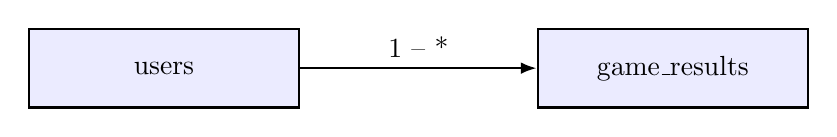
\begin{tikzpicture}[node distance=3cm]
    \tikzstyle{entity} = [rectangle, draw=black, thick, fill=blue!8,
        text width=3.2cm, align=center, minimum height=1cm]
    \node (users) [entity] {users};
    \node (results) [entity, right=of users] {game\_results};
    \draw [-{Latex[length=2mm]}, thick] (users) -- node[above] {1 -- *} (results);
\end{tikzpicture}
\caption{Entity relationship between \texttt{users} and \texttt{game\_results}.}
\label{fig:er-diagram}
\end{figure}

\section{Important Constraints}
\begin{itemize}[nosep]
    \item Foreign key: \texttt{game\_results.user\_id} references
    \texttt{users.id}.
    \item Unique constraints on \texttt{users.username} and
    \texttt{users.email} prevent duplicate accounts.
    \item ENUM constraint on \texttt{game\_results.difficulty} restricts the
    column to exactly \texttt{beginner} or \texttt{advanced}.
    \item An index is defined on \texttt{game\_results.user\_id} (and on
    \texttt{score} for leaderboard ordering) to support efficient history
    and ranking queries.
\end{itemize}

\section{Schema Evolution}
An early version of the schema included a \texttt{result} column recording
a win/loss outcome, consistent with a classic ``clear the board'' win
condition. When the game was redesigned as a timed survival mode
(Section~\textit{Survival Mode and the Absence of a Win Condition},
Chapter~\ref{ch:game-design}), this column was no longer meaningful and was
removed via \texttt{migration-remove-win-condition.sql}, since a completed
game is now fully described by its difficulty, time survived, cells
revealed, and hints used.

\chapter{Implementation}
\label{ch:implementation}

\section{Frontend Implementation}
The frontend is built with React and bundled with Vite, using plain
JavaScript (no TypeScript) and component-scoped CSS. No external UI
component framework is used for the game board itself; the board is
rendered as a CSS grid of cell components, each responding to left-click
(reveal), right-click (flag), and, on an already-revealed numbered cell,
click-again (chord).

\section{Backend Implementation}
The backend is written in procedural PHP, without a framework, as a
collection of standalone endpoint scripts plus shared includes for the
database connection and authentication helpers. Unlike a typical
\texttt{mysqli}-based implementation, database access uses PHP's PDO
extension with prepared statements throughout, so that every query
involving user-supplied data is parameterized.

\section{API Endpoints}
Table~\ref{tab:api-endpoints} summarises the backend endpoints exposed by
the application.

\begin{table}[h]
\centering
\caption{Summary of backend API endpoints.}
\label{tab:api-endpoints}
\begin{tabular}{@{}p{3.4cm}p{1.6cm}p{1.8cm}p{6.5cm}@{}}
\toprule
\textbf{Endpoint} & \textbf{Method} & \textbf{Auth} & \textbf{Purpose} \\
\midrule
register.php & POST & No & Create a new user account \\
login.php & POST & No & Authenticate and start a session \\
logout.php & POST & Yes & Destroy the current session \\
save-score.php & POST & Yes & Recompute and persist a completed game's result \\
leaderboard.php & GET & Yes & Return the top scores, optionally filtered by difficulty \\
history.php & GET & Yes & Return the logged-in user's past games \\
stats.php & GET & Yes & Return the logged-in user's aggregate statistics \\
\bottomrule
\end{tabular}
\end{table}

\section{Representative Frontend Code: API Wrapper}
\begin{lstlisting}[language=JavaScript, caption={Simplified fetch wrapper (\texttt{services/api.js}).}, label={lst:api-js}]
const API_BASE = import.meta.env.VITE_API_URL;

export async function apiRequest(endpoint, options = {}) {
  const response = await fetch(`${API_BASE}${endpoint}`, {
    credentials: "include",
    headers: { "Content-Type": "application/json" },
    ...options,
  });
  const data = await response.json();
  if (!response.ok || !data.success) {
    throw new Error(data.message || "Request failed");
  }
  return data;
}
\end{lstlisting}

\section{Representative Backend Code: Score Submission Endpoint}
\texttt{save-score.php} is the most security-relevant endpoint in the
system, since it is the only point at which client-reported gameplay
metrics are converted into a persisted, leaderboard-visible score. Its
validation logic is described fully in Section~\ref{sec:score-validation}
of Chapter~\ref{ch:security}; a simplified outline is shown below.

\begin{lstlisting}[language=PHP, caption={Simplified score submission endpoint (\texttt{save-score.php}).}, label={lst:save-score}]
<?php
require_once "includes/db.php";
require_once "includes/auth.php";
require_login();

$input = json_decode(file_get_contents("php://input"), true);
$difficulty = $input["difficulty"];
$timeTaken = (int) $input["time_taken"];
$cellsRevealed = (int) $input["cells_revealed"];
$hintsUsed = (int) $input["hints_used"];

// Bound-check against the known limits for this difficulty
validate_metrics($difficulty, $timeTaken, $cellsRevealed, $hintsUsed);

// Reject if an identical result was submitted in the last 10 seconds
reject_if_duplicate($userId, $difficulty, $timeTaken, $cellsRevealed, $hintsUsed);

// Recompute the score server-side; never trust a client-supplied score
$score = max(0, $cellsRevealed * 10 - $hintsUsed * 50);

$stmt = $pdo->prepare(
  "INSERT INTO game_results (user_id, difficulty, score, time_taken, cells_revealed, hints_used)
   VALUES (?, ?, ?, ?, ?, ?)"
);
$stmt->execute([$userId, $difficulty, $score, $timeTaken, $cellsRevealed, $hintsUsed]);
\end{lstlisting}

\section{Configuration Management}
Difficulty parameters are defined once on the frontend in the
\texttt{DIFFICULTIES} configuration object (grid size and mine count) and
independently on the backend as the bounds used by
\texttt{validate\_metrics()} (maximum safe cells per difficulty). This
duplication -- rather than a single shared source of truth -- is noted as a
maintainability limitation in Chapter~\ref{ch:limitations}.

\chapter{Security}
\label{ch:security}

Security is treated as a dedicated chapter because the project's central
integrity concern -- preventing a client from fabricating a game result --
is addressed through a specific set of server-side mechanisms that go beyond
generic web-application hardening.

\section{Password Storage}
Passwords are hashed at registration time with
\texttt{password\_hash(\$password, PASSWORD\_DEFAULT)} and verified at login
time with \texttt{password\_verify()}. Plaintext passwords are never stored
or logged.

\section{Session Security}
\label{sec:session-security}
Authentication is session-based, using PHP's native session mechanism.
\begin{itemize}[nosep]
    \item \textbf{Session fixation mitigation} -- on successful login, the
    session ID is regenerated with \texttt{session\_regenerate\_id(true)},
    preventing an attacker from fixing a victim's session ID before login.
    \item \textbf{Cookie hardening} -- the session cookie is configured as
    HTTP-only (inaccessible to client-side JavaScript), with
    \texttt{SameSite=Lax} and scoped to the application's domain.
    \item \textbf{Server-side authorization} -- every protected endpoint
    calls a shared \texttt{require\_login()} helper that checks for a valid
    session before performing any work, independent of any client-side
    route guard (Chapter~\ref{ch:architecture}).
\end{itemize}

\section{Cross-Origin Resource Sharing (CORS)}
The backend restricts cross-origin requests to an explicit allow-list of
known frontend origins, checked against the request's \texttt{Origin}
header, rather than reflecting an arbitrary origin or using a wildcard.
This is required because the frontend (Vite dev server / deployed SPA) and
backend are served from different origins, and CORS must be configured
correctly for the session cookie to be sent and accepted.

\section{SQL Injection Prevention}
All database access uses PDO prepared statements with bound parameters. No
endpoint concatenates user-supplied input directly into a SQL string.

\section{Server-Side Score Validation}
\label{sec:score-validation}
Because the game engine runs entirely on the client
(Chapter~\ref{ch:game-design}), the score value computed in the browser
during play is treated as untrusted input. \texttt{save-score.php}
recomputes the score independently from the raw submitted metrics
(\texttt{cells\_revealed}, \texttt{time\_taken}, \texttt{hints\_used}) using
the same formula described in Section~\ref{sec:scoring}, and additionally
bounds each metric against the known limits for the submitted difficulty
(for example, \texttt{cells\_revealed} cannot exceed the total safe-cell
count for that difficulty, and \texttt{hints\_used} cannot exceed 3). A
submission whose metrics fall outside these bounds is rejected. This means
the value shown to the player at the end of a game is never the value
actually written to the \texttt{game\_results} table or shown on the
leaderboard; the stored value is always the server's own computation.

\section{Duplicate / Replay Submission Defense}
To reduce the risk of the same completed game being submitted multiple
times (whether accidentally or as a deliberate replay attempt), the backend
computes a signature over the combination of user ID, difficulty, time
taken, cells revealed, and hints used (an MD5 digest of the concatenated
values), and rejects a new submission that matches a previous submission's
signature within a 10-second window. This is a heuristic defense rather
than a cryptographically strong nonce or idempotency-key mechanism; its
scope and limitations are discussed further in
Chapter~\ref{ch:limitations}.

\section{Security Measures Summary}
\begin{table}[h]
\centering
\caption{Summary of applied security measures.}
\label{tab:security-summary}
\begin{tabular}{@{}p{4.2cm}p{9.5cm}@{}}
\toprule
\textbf{Measure} & \textbf{Purpose} \\
\midrule
Bcrypt password hashing & Prevent plaintext password exposure on data breach \\
Session ID regeneration on login & Mitigate session fixation attacks \\
HTTP-only, SameSite cookies & Reduce cookie theft via XSS / cross-site request risk \\
CORS origin allow-list & Prevent arbitrary origins from making authenticated requests \\
PDO prepared statements & Prevent SQL injection \\
Server-side score recomputation & Prevent client-fabricated leaderboard scores \\
Metric bounds checking & Prevent out-of-range or impossible gameplay metrics \\
Duplicate-submission signature & Reduce accidental/duplicate or naive replay submissions \\
\bottomrule
\end{tabular}
\end{table}

\section{Known Absences}
For completeness, and in the same spirit of honest disclosure as the
security chapter of the reference report, the following protections are
\emph{not} currently implemented: CSRF tokens on state-changing POST
requests, request rate limiting, and enforced HTTPS in the development
configuration (the session cookie's \texttt{secure} flag is \texttt{false}
in the current setup). These are discussed further in
Chapter~\ref{ch:limitations}.

\chapter{User Interface and Major Features}
\label{ch:ui-features}

\section{Page Walkthrough}

\subsection{Login and Registration}
The login page (Figure~\ref{fig:ui-login}) collects an email address and
password. The registration page (Figure~\ref{fig:ui-register}) collects a
username, email, password, and password confirmation, and links back to the
login page for existing users.

\begin{figure}[h]
    \centering
    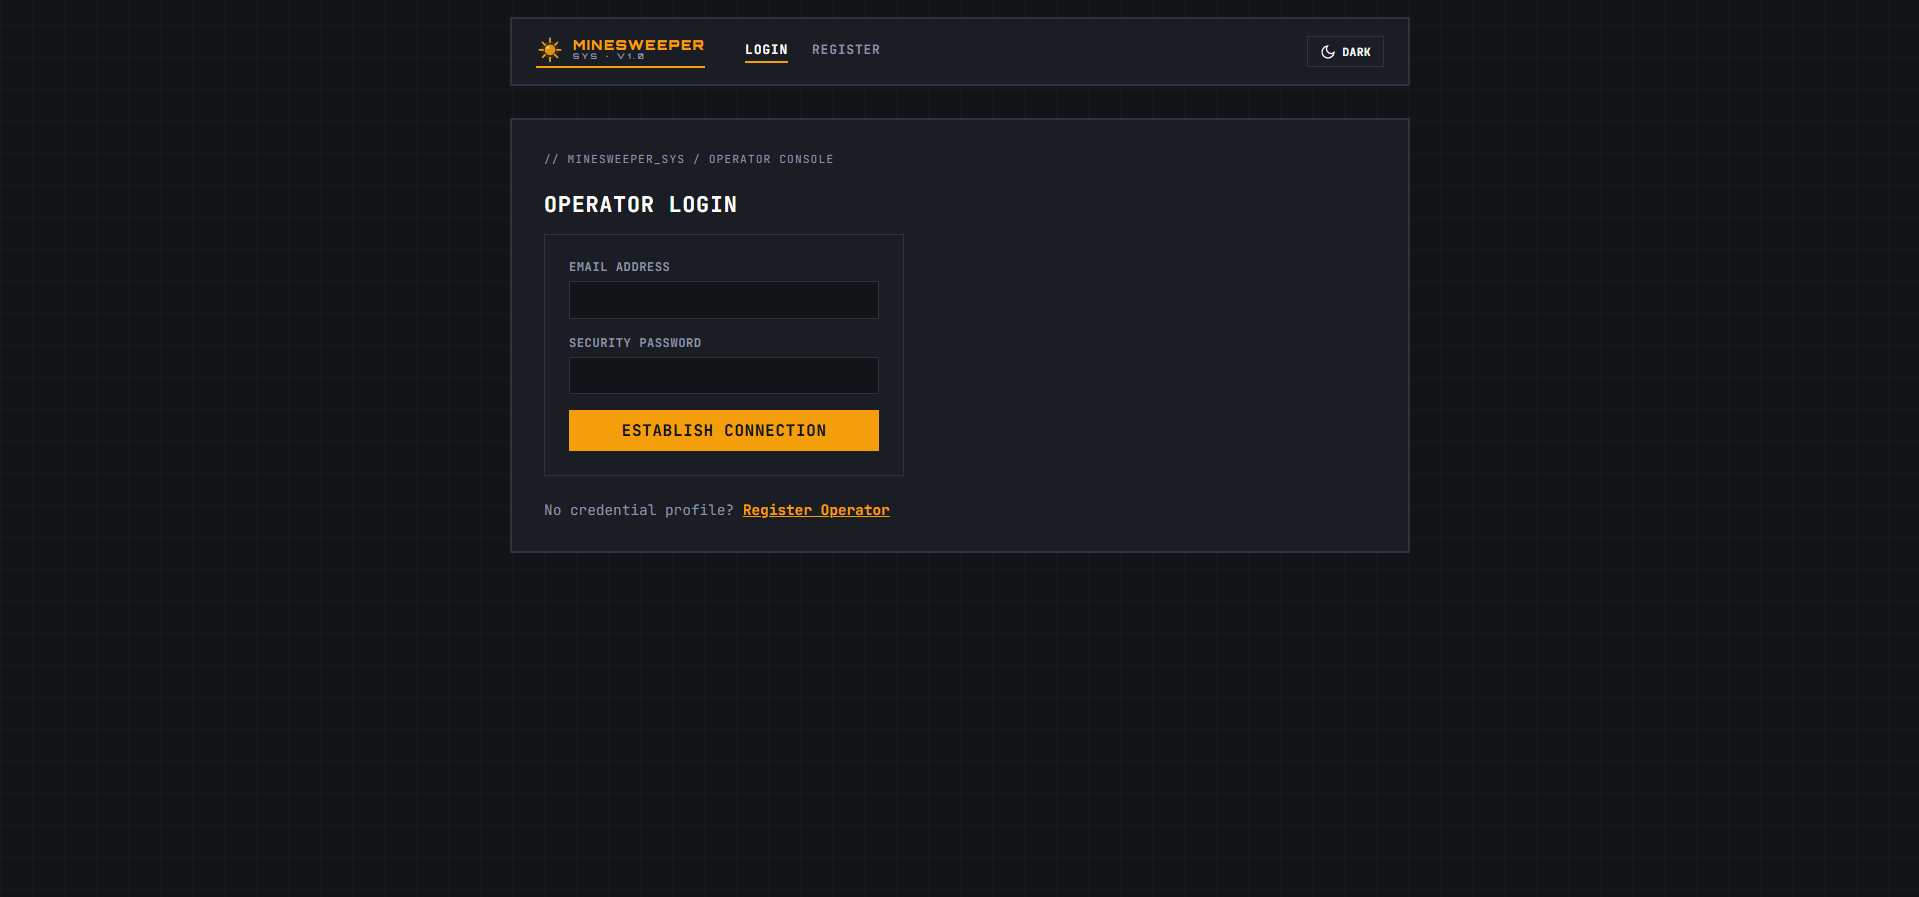
\includegraphics[width=0.8\textwidth]{figures/fig_login.png}
    \caption{Login page (dark theme).}
    \label{fig:ui-login}
\end{figure}

\begin{figure}[h]
    \centering
    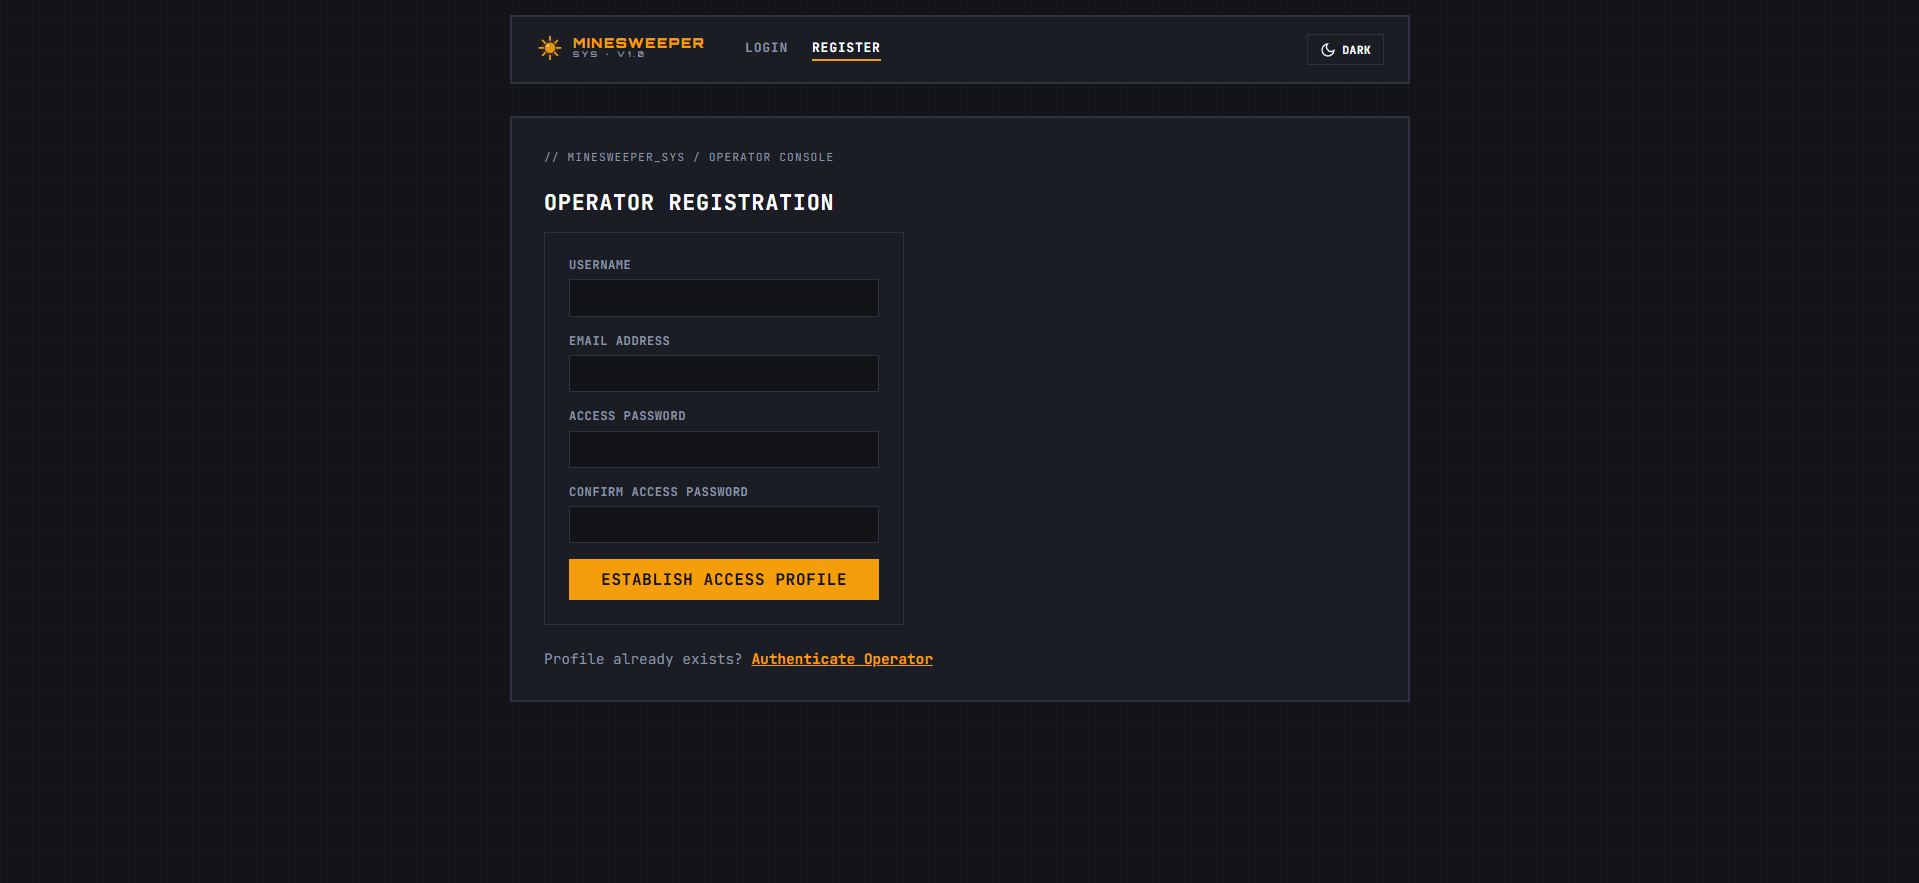
\includegraphics[width=0.8\textwidth]{figures/fig_register.png}
    \caption{Registration page (dark theme).}
    \label{fig:ui-register}
\end{figure}

\subsection{Dashboard}
The dashboard (Figures~\ref{fig:ui-dashboard-dark}
and~\ref{fig:ui-dashboard-light}) is the player's home screen. It shows the
player's identity, a set of aggregate statistics (games played, high score,
average score, longest survival time, most cells revealed), filterable by
"All Modes", "Beginner", or "Advanced", and quick-access links to the
dashboard, game history, leaderboard, and a new game.

\begin{figure}[h]
    \centering
    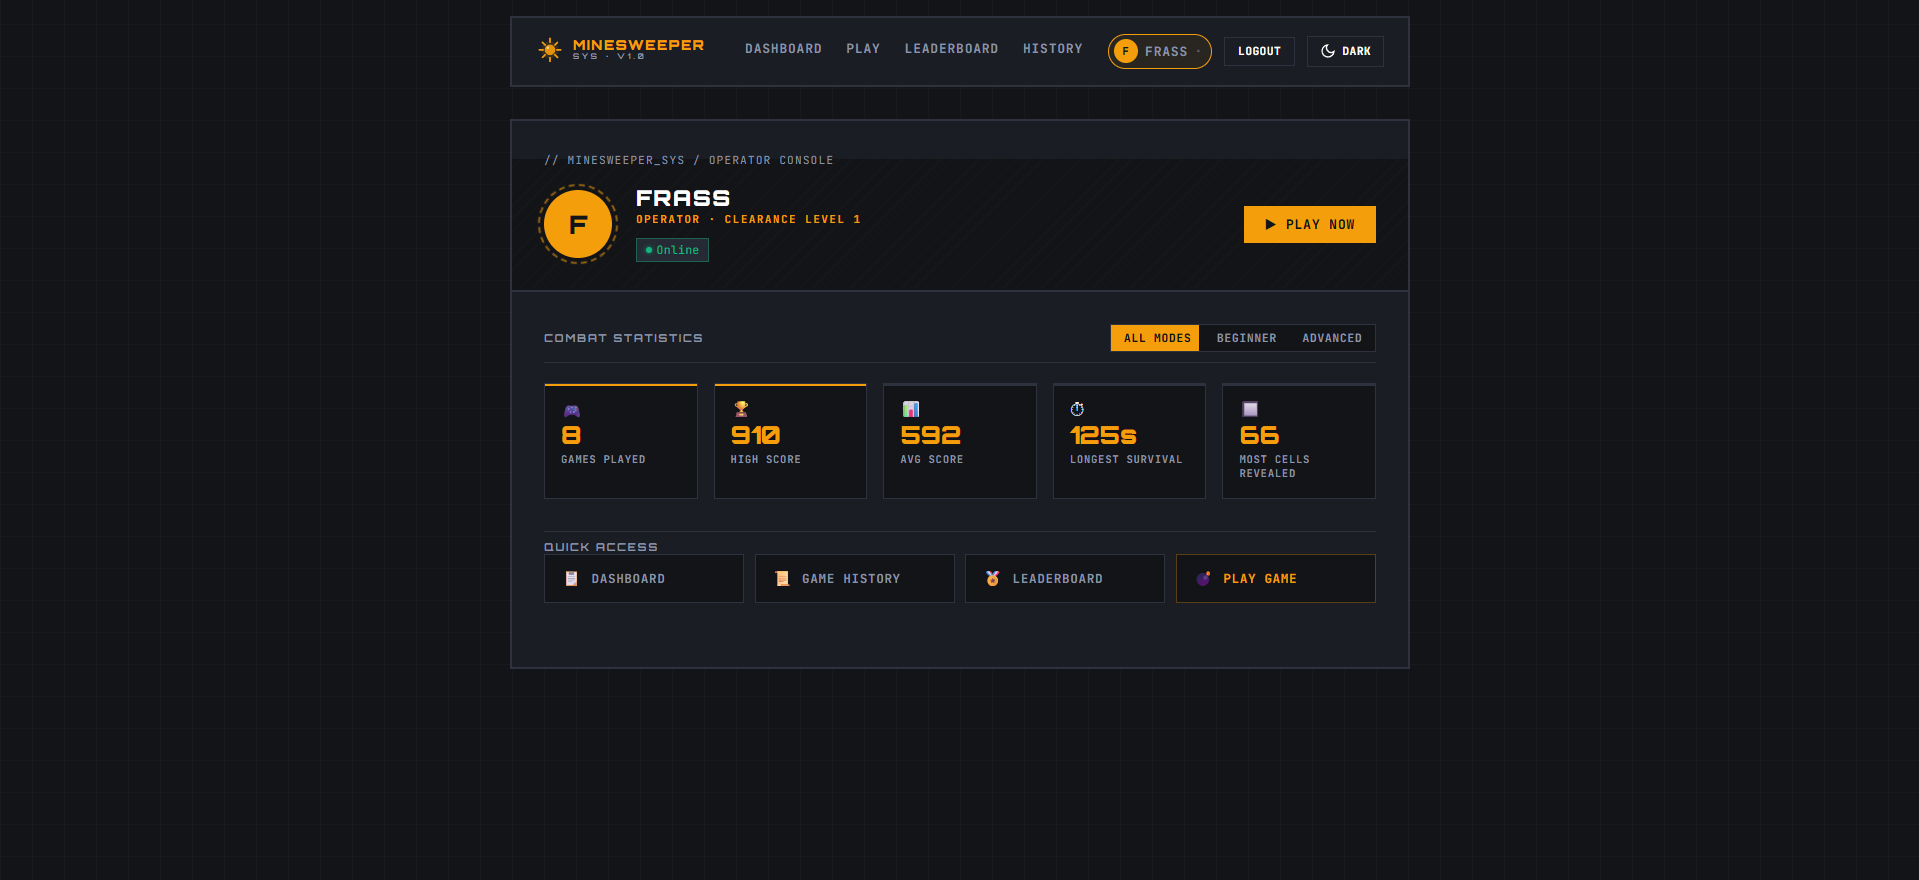
\includegraphics[width=0.8\textwidth]{figures/fig_profile_dark.png}
    \caption{Player dashboard with combat statistics (dark theme).}
    \label{fig:ui-dashboard-dark}
\end{figure}

\begin{figure}[h]
    \centering
    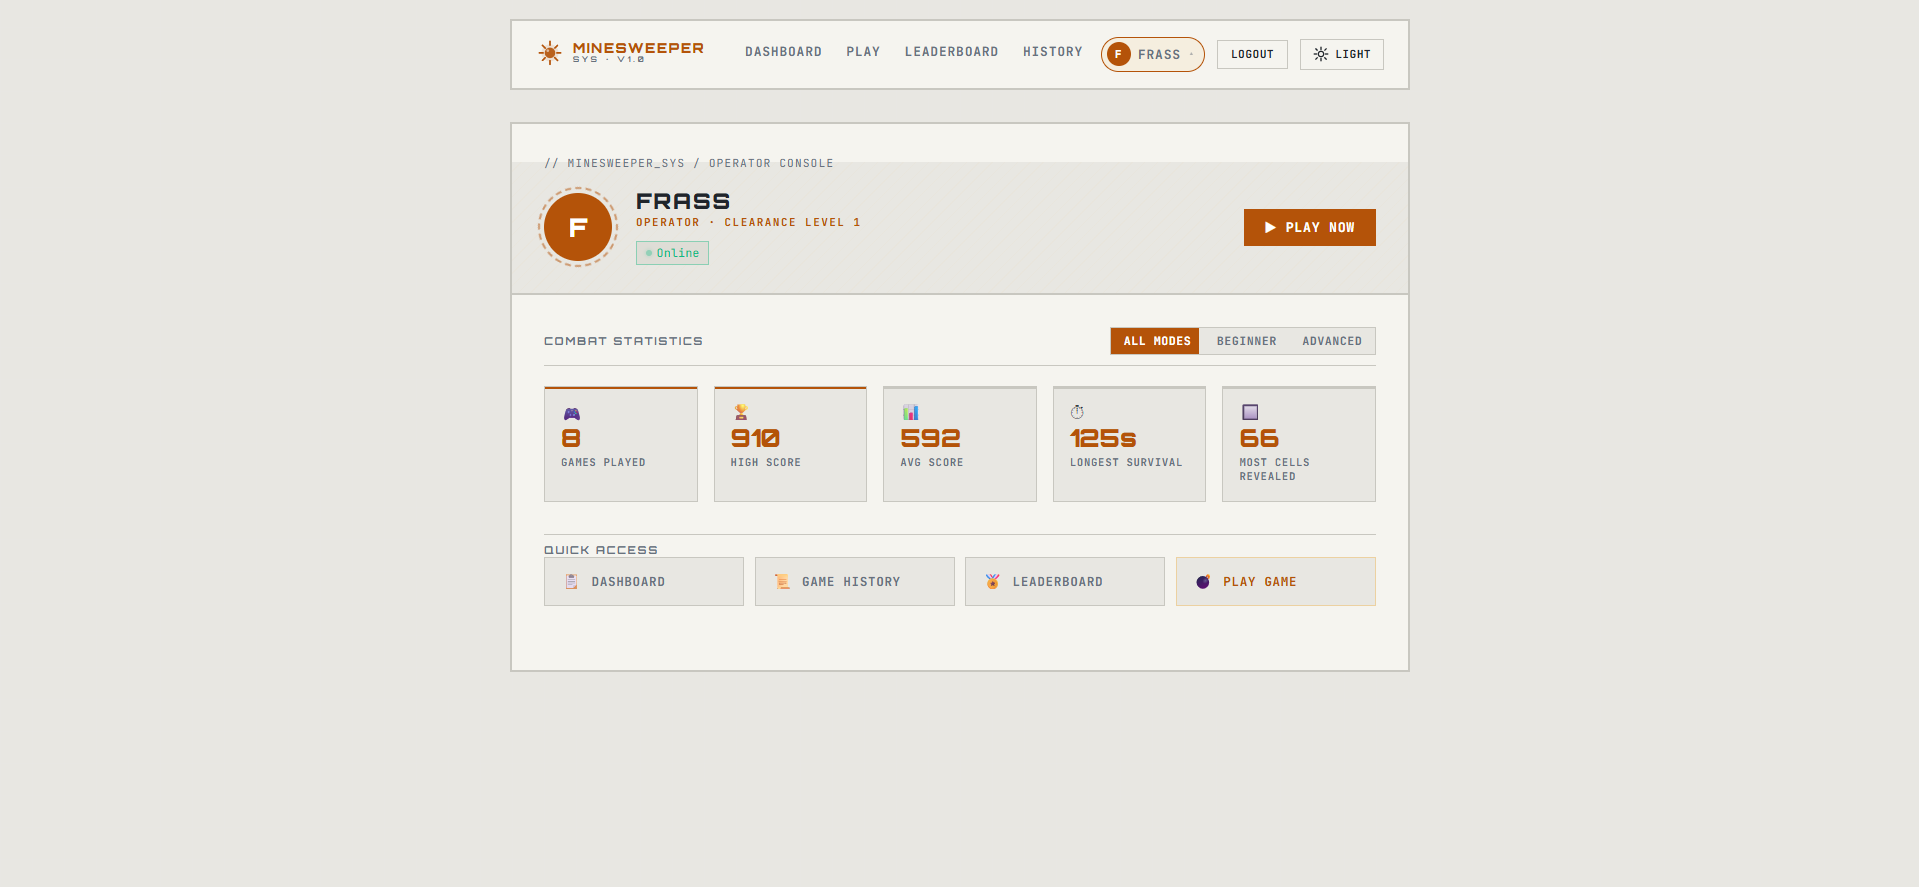
\includegraphics[width=0.8\textwidth]{figures/fig_profile_light.png}
    \caption{Player dashboard with combat statistics (light theme), showing
    theme support.}
    \label{fig:ui-dashboard-light}
\end{figure}

\subsection{Game Page}
The game page (Figure~\ref{fig:ui-game}) shows a difficulty selector
(Beginner / Advanced), the current mine count, flag count, and score, a
countdown timer, the interactive board itself, a hint button showing
remaining hints, a restart button, and the shield control with its current
state (\emph{Ready}, \emph{Active}, or \emph{Used}).

\begin{figure}[h]
    \centering
    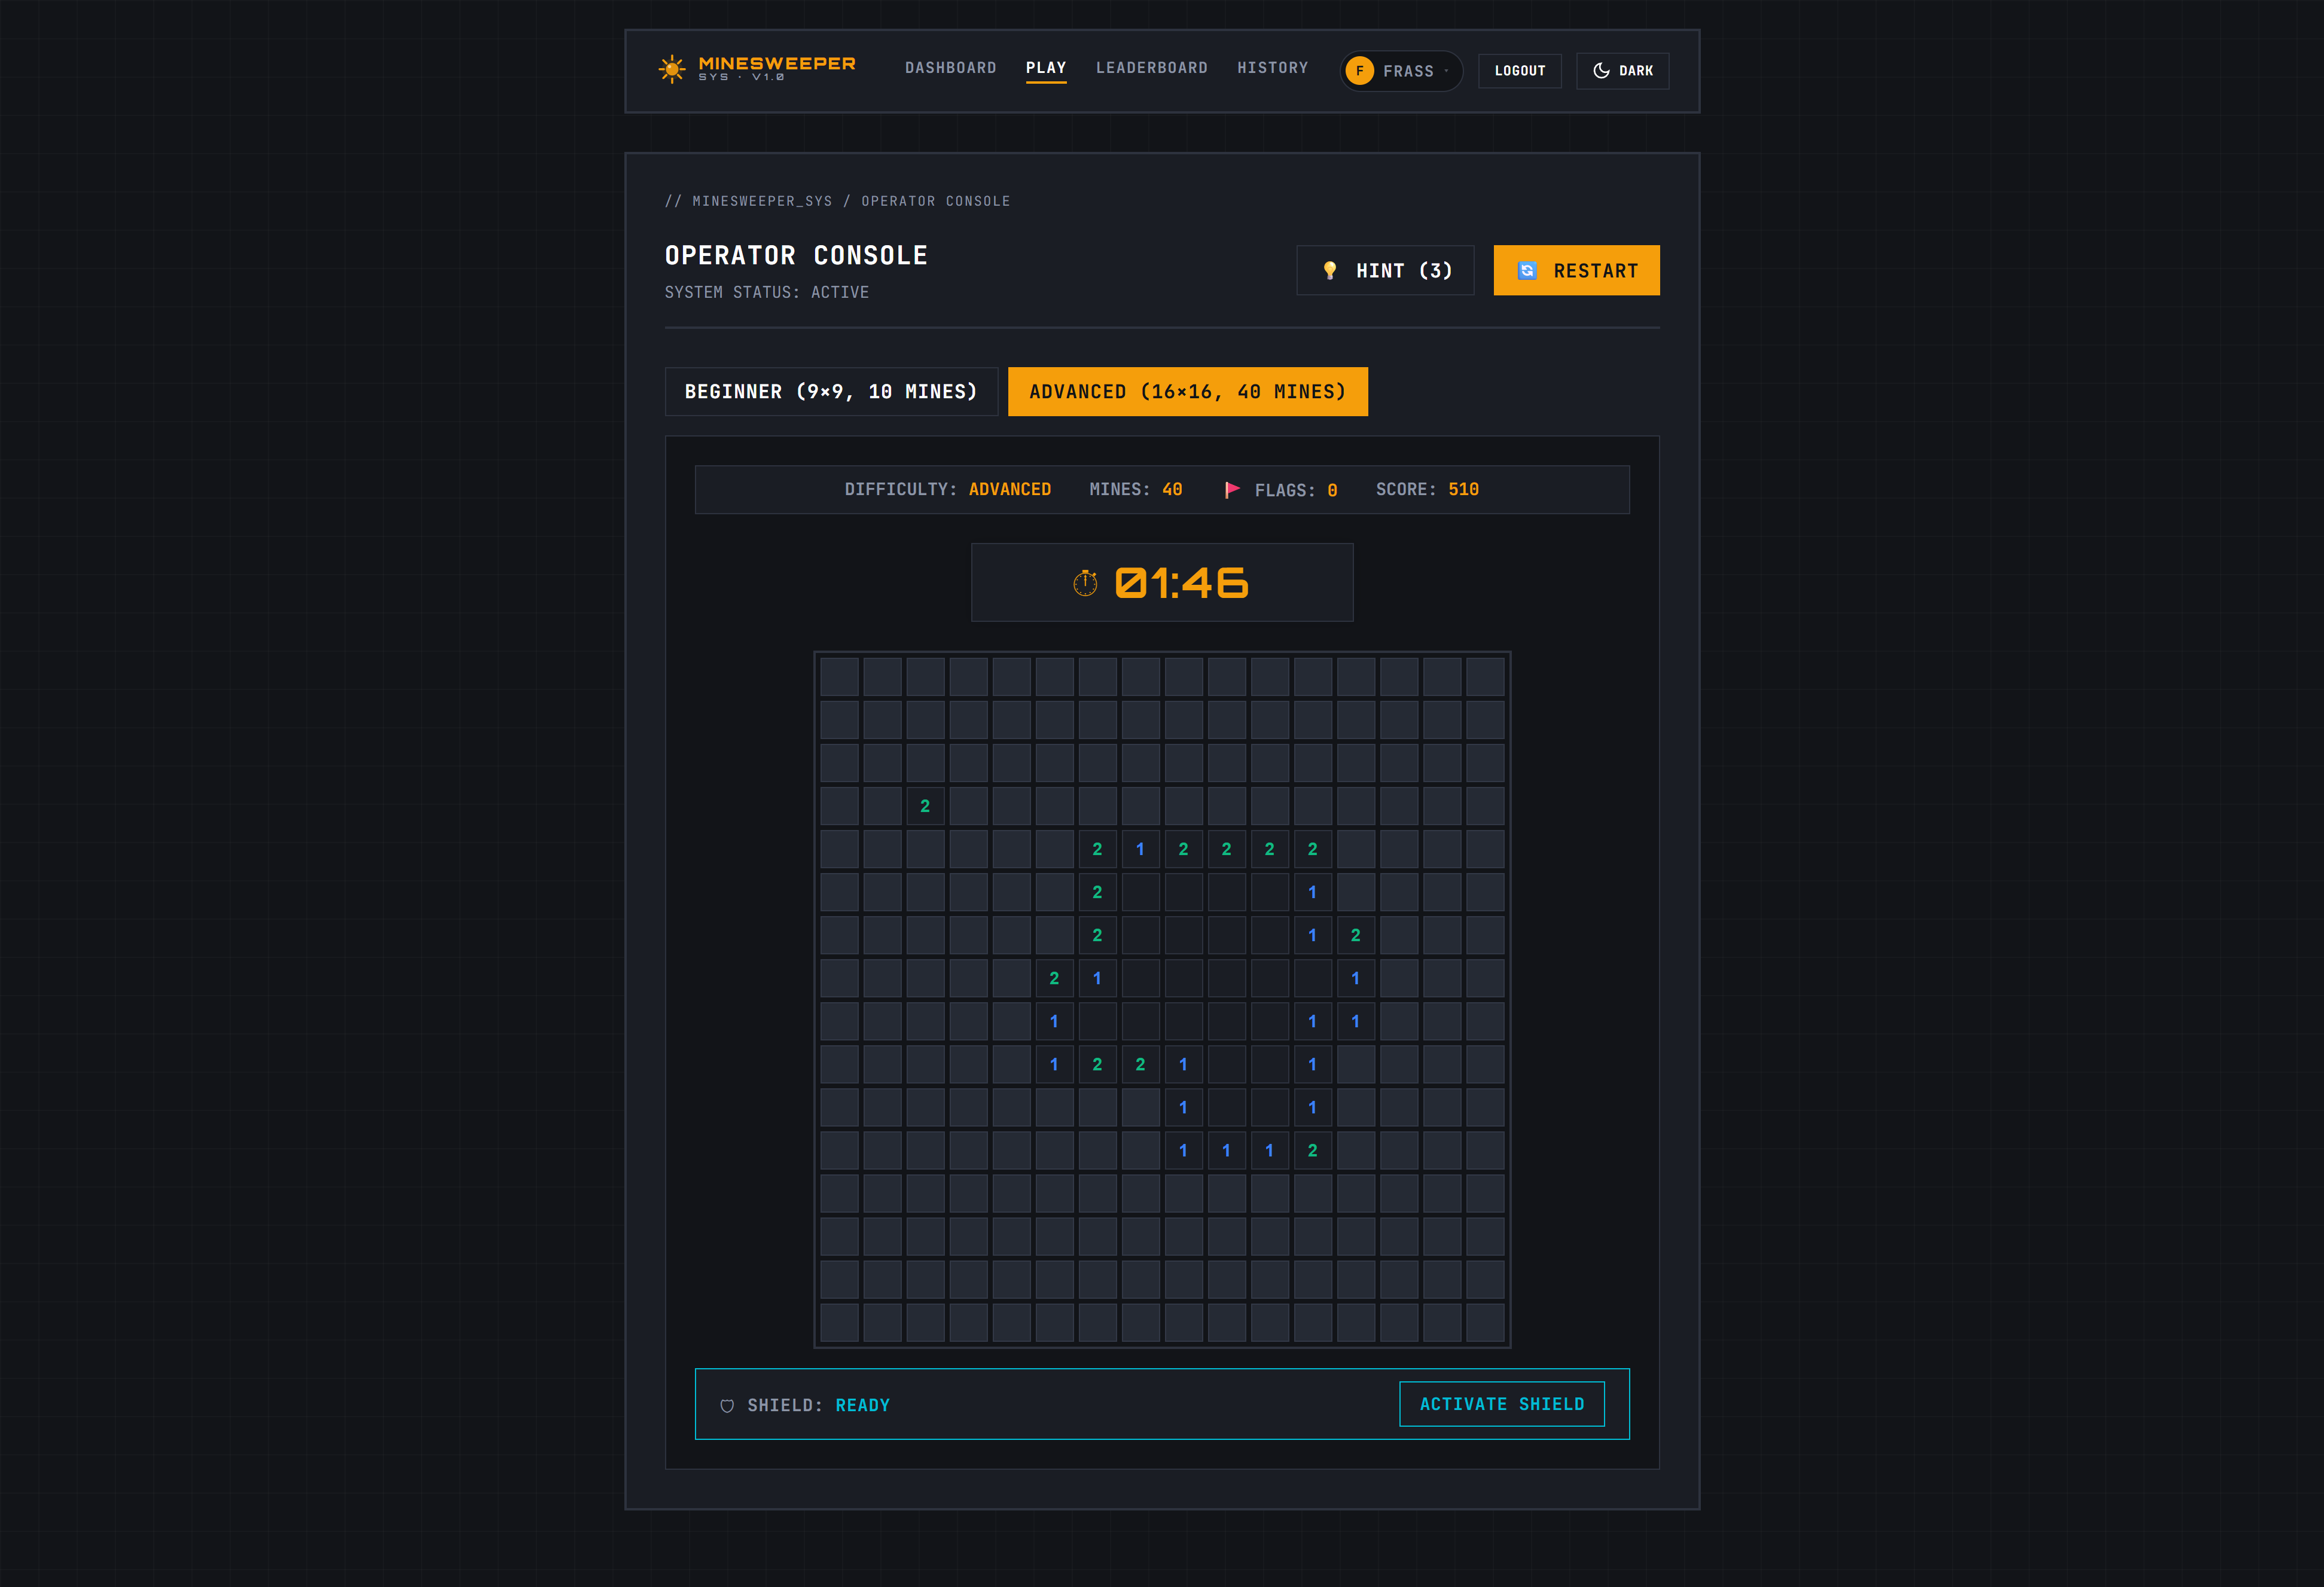
\includegraphics[width=0.85\textwidth]{figures/fig_game_board.png}
    \caption{Active game on Advanced difficulty, showing the timer, score,
    flag count, partially revealed board, and shield control.}
    \label{fig:ui-game}
\end{figure}

\subsection{Leaderboard}
The leaderboard page (Figure~\ref{fig:ui-leaderboard}) lists the top scores
across all players, filterable by "All", "Beginner", or "Advanced", with
columns for rank, player, difficulty, score, time, cells revealed, and
hints used.

\begin{figure}[h]
    \centering
    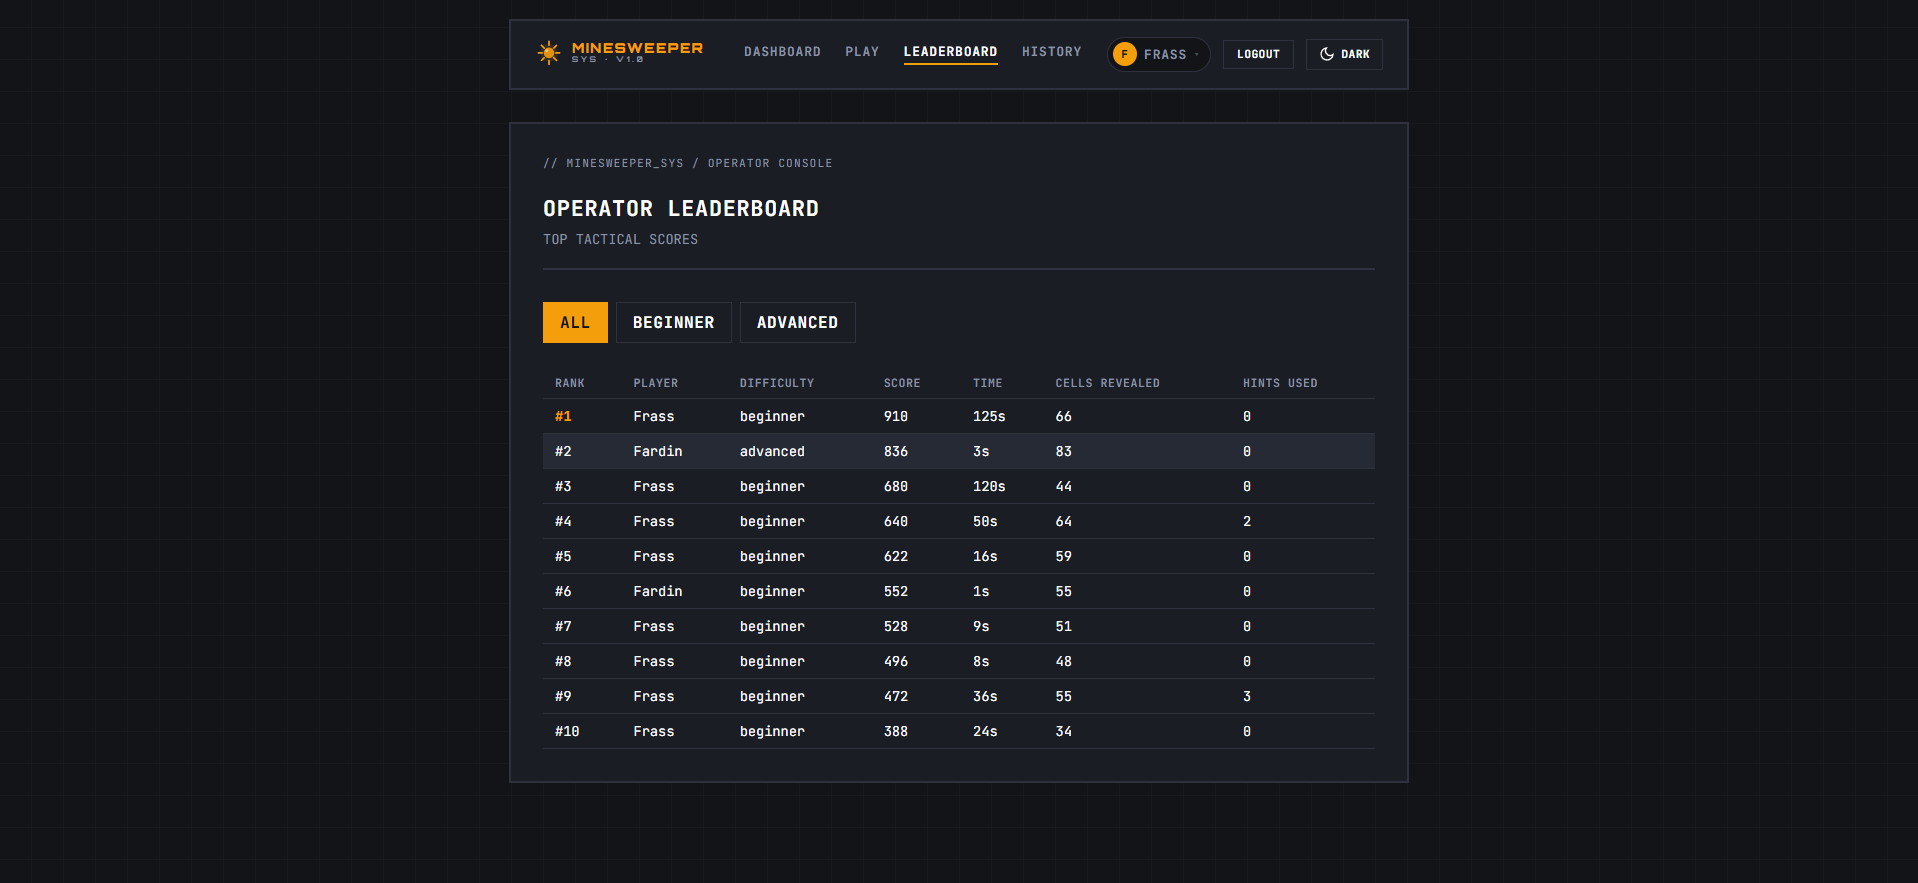
\includegraphics[width=0.85\textwidth]{figures/fig_leaderboard.png}
    \caption{Global leaderboard, filtered to all difficulties.}
    \label{fig:ui-leaderboard}
\end{figure}

\subsection{History}
The history page (Figure~\ref{fig:ui-history}) lists the logged-in player's
own past completed games, newest first, with the same metric columns as the
leaderboard.

\begin{figure}[h]
    \centering
    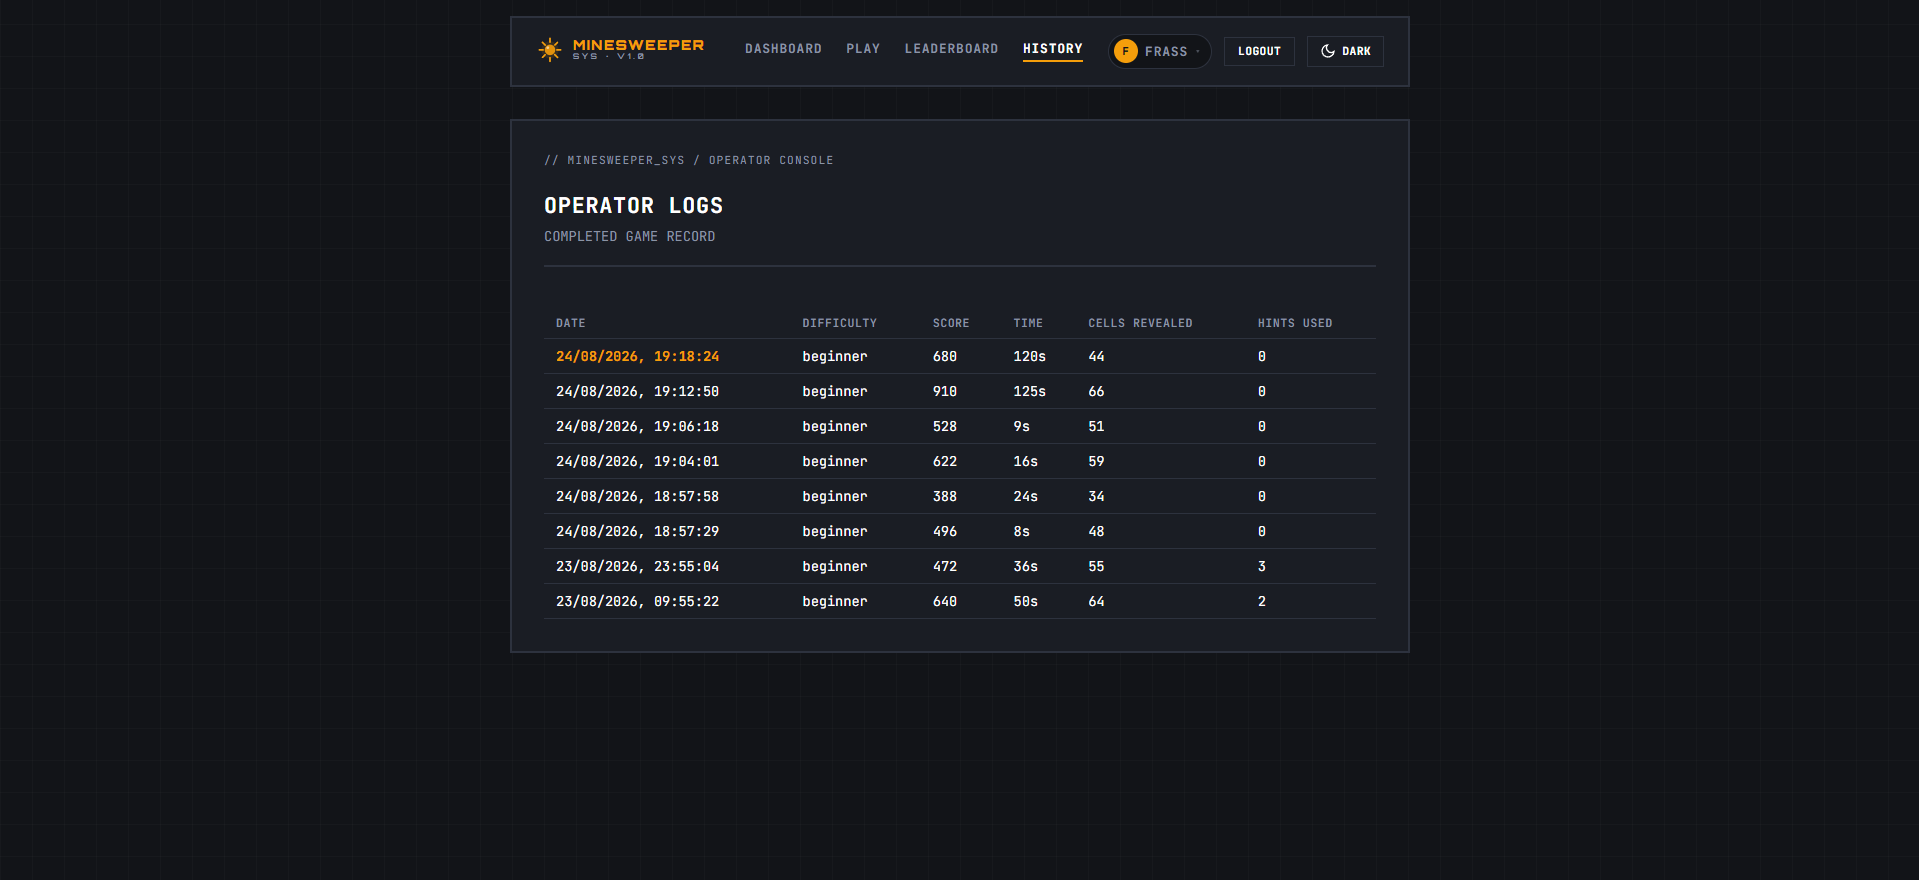
\includegraphics[width=0.85\textwidth]{figures/fig_history.png}
    \caption{Player's personal game history.}
    \label{fig:ui-history}
\end{figure}

\section{Theme Support}
The application supports light and dark themes, toggled from the navigation
bar and managed through \texttt{ThemeContext}. Figures~\ref{fig:ui-dashboard-dark}
and~\ref{fig:ui-dashboard-light} show the same dashboard rendered in both
themes.

\section{Feature Summary}

\begin{table}[h]
\centering
\caption{Core gameplay features.}
\label{tab:core-features}
\begin{tabular}{@{}p{4cm}p{9.5cm}@{}}
\toprule
\textbf{Feature} & \textbf{Description} \\
\midrule
Two difficulties & Beginner ($9\times9$, 10 mines) and Advanced ($16\times16$, 40 mines) \\
First-click safety & Guaranteed-safe first reveal and its neighbourhood \\
Flood-fill reveal & Automatic cascading reveal of zero-adjacency regions \\
Flagging & Mark/unmark suspected mine cells, capped at the mine count \\
Chording & Reveal all unflagged neighbours of a satisfied numbered cell \\
Hints & Up to 3 random safe-cell highlights per game, at a score cost \\
Shield & One-time protection against the next mine reveal \\
Survival timer & 120-second countdown; game ends on mine or timeout \\
Live scoring & Score recalculated and displayed during play \\
\bottomrule
\end{tabular}
\end{table}

\begin{table}[h]
\centering
\caption{Account and meta features.}
\label{tab:meta-features}
\begin{tabular}{@{}p{4cm}p{9.5cm}@{}}
\toprule
\textbf{Feature} & \textbf{Description} \\
\midrule
Registration / Login / Logout & Session-based account management \\
Personal dashboard & Aggregate statistics, filterable by difficulty \\
Game history & Full list of the player's own past completed games \\
Global leaderboard & Top scores across all players, filterable by difficulty \\
Theme support & Light/dark theme toggle \\
\bottomrule
\end{tabular}
\end{table}

\chapter{Testing and Validation}
\label{ch:testing}

\section{Test Strategy}
The system was validated using a structured, manual, black-box test plan,
covering account management, the core game algorithms, server-side score
validation, and cross-cutting security behaviours. Each test case specifies
the steps to perform and the expected result, so the system's observable
behaviour can be checked directly against the requirements in
Chapter~\ref{ch:requirements}.

\section{Test Cases}
Table~\ref{tab:test-cases} lists the test cases referenced by the
requirements-traceability table in Chapter~\ref{ch:requirements}, along with
additional representative cases covering the game engine and security
mechanisms.

\begin{table}[h]
\centering
\caption{Representative functional and security test cases.}
\label{tab:test-cases}
\begin{tabular}{@{}p{1.2cm}p{5.3cm}p{6.2cm}@{}}
\toprule
\textbf{ID} & \textbf{Steps} & \textbf{Expected Result} \\
\midrule
T-1 & Register with a password under 6 characters. & Registration rejected with a validation error; no account created. \\
T-2 & Inspect the stored password value after registration. & Value is a bcrypt hash, not the plaintext password. \\
T-3 & Log in with the correct email but an incorrect password. & Login rejected; session not created. \\
T-4 & Start a game and click any cell as the first move. & The clicked cell and all of its neighbours are guaranteed not to be mines. \\
T-5 & Click a cell with zero adjacent mines. & All connected zero-adjacency cells, and their numbered border, are revealed in one action. \\
T-6 & Flag the correct number of mines around a revealed numbered cell, then click it again. & All remaining unflagged neighbours are revealed at once (chord). \\
T-7 & Activate the shield, then reveal a mine. & The game continues; the shield becomes \emph{used}; the mine is not revealed as a loss. \\
T-8 & Use all 3 hints in a single game. & The 4th hint request is not granted; each used hint reduces the final score by 50 points. \\
T-9 & Submit a manually crafted request to \texttt{save-score.php} with an inflated \texttt{cells\_revealed} value. & Request is rejected for exceeding the valid bound for the given difficulty. \\
T-10 & Submit the same result twice within 10 seconds. & The second submission is rejected as a duplicate. \\
T-11 & Log in as one user, then attempt to request another user's history via the API. & Only the authenticated user's own data is returned. \\
T-12 & Attempt a classic SQL injection payload in the login form. & Login fails cleanly; no database error is exposed. \\
T-13 & Let the timer reach zero without hitting a mine. & Game ends, all mines are revealed, and the result is submitted automatically. \\
\bottomrule
\end{tabular}
\end{table}

\section{Security Tests}
Security-focused testing specifically targeted the mechanisms described in
Chapter~\ref{ch:security}:
\begin{itemize}[nosep]
    \item \textbf{SQL injection resistance} (T-12) -- confirmed that
    injection payloads in the login form fail cleanly, since all queries use
    PDO prepared statements.
    \item \textbf{Score tampering resistance} (T-9) -- confirmed that
    metrics outside the valid range for a difficulty are rejected rather
    than trusted.
    \item \textbf{Duplicate submission resistance} (T-10) -- confirmed that
    an identical result submitted twice in quick succession is rejected the
    second time.
    \item \textbf{Cross-user data isolation} (T-11) -- confirmed that a
    user's history and statistics endpoints only ever return that user's own
    data, based on the server-side session rather than any client-supplied
    identifier.
\end{itemize}

\section{Results}
All test cases described above passed against the described behaviour of
the system at the time of testing: first-click safety, flood-fill, and
chording behave correctly across repeated trials; the shield correctly
absorbs exactly one mine reveal per game; hints are capped at 3 and reduce
the final score as expected; and the server-side score validation and
duplicate-submission checks were both exercised successfully against
manually crafted requests.

\chapter{Results and Discussion}
\label{ch:results}

The completed application successfully implements a browser-playable
Minesweeper game with persistent accounts, a global leaderboard, personal
statistics, and game history, on top of a game engine that runs entirely on
the client. In its current form, the system:

\begin{itemize}[nosep]
    \item Correctly guarantees a safe first click and its neighbourhood on
    every new game, regardless of difficulty.
    \item Correctly cascades reveals through zero-adjacency regions using an
    iterative, non-recursive flood-fill, avoiding recursion-depth concerns
    on the larger $16\times16$ Advanced board.
    \item Supports chording and a single-use shield ability as additional
    layers of player strategy beyond classic reveal/flag play.
    \item Enforces a strict separation between client-side gameplay and
    server-side score authority: the score shown to the player during play
    is never the value trusted for the leaderboard, which is instead
    recomputed and bounds-checked independently by \texttt{save-score.php}.
    \item Presents personal statistics, a full game history, and a global
    leaderboard, each filterable by difficulty, giving the player both
    short-term feedback and long-term progress tracking.
\end{itemize}

The decision to implement the game engine as a set of pure, testable
functions (\texttt{minesweeper.js}), separate from the React state
management in \texttt{useMinesweeper.js}, kept the core algorithms
(first-click safety, flood-fill, chording, scoring) independent of the UI
framework and straightforward to reason about and validate directly, as
reflected in the test cases in Chapter~\ref{ch:testing}. Likewise, treating
the client-computed score as untrusted input and recomputing it
server-side, rather than simply persisting whatever the client reports,
directly addresses the score-integrity problem identified in the
Introduction (Chapter~\ref{ch:introduction}).

The use of a single-page React frontend against a lightweight,
framework-free procedural PHP API kept the backend small and easy to audit,
while still demonstrating a complete client-server-database pipeline with
real authentication, authorization, and data-integrity concerns, which
suited the goals of the project.

\chapter{Limitations}
\label{ch:limitations}

\begin{itemize}[nosep]
    \item \textbf{No CSRF protection} -- state-changing POST requests
    (e.g.\ \texttt{save-score.php}, \texttt{logout.php}) do not carry a CSRF
    token, relying instead on the CORS origin allow-list and SameSite
    cookie policy as the primary cross-site defenses.
    \item \textbf{Heuristic duplicate-submission signature} -- the
    duplicate-submission check (Section~\ref{sec:score-validation}) uses an
    MD5 digest of the submitted metrics and a 10-second window rather than a
    cryptographically strong, single-use nonce; a sufficiently patient or
    varied replay could still evade it.
    \item \textbf{Development-mode cookie configuration} -- the session
    cookie's \texttt{secure} flag is currently \texttt{false}, appropriate
    for local HTTP development but not for a production HTTPS deployment.
    \item \textbf{Duplicated difficulty configuration} -- the grid size and
    mine count for each difficulty are defined independently on the
    frontend (\texttt{DIFFICULTIES}) and as validation bounds on the backend
    (\texttt{validate\_metrics()}), rather than from a single shared source
    of truth, so the two must be kept manually in sync.
    \item \textbf{No password reset flow} -- a user who forgets their
    password has no self-service recovery mechanism.
    \item \textbf{Leaderboard scope} -- the leaderboard displays a fixed
    top-10 list without pagination.
    \item \textbf{No rate limiting} -- login and registration endpoints do
    not throttle repeated requests, leaving them potentially susceptible to
    brute-force attempts.
    \item \textbf{No formal foreign-key-backed role separation} -- since
    there is only one user role, this is not currently a concern, but it is
    noted as a constraint on any future addition of privileged accounts.
\end{itemize}

\chapter{Future Enhancements}
\label{ch:future}

\begin{itemize}[nosep]
    \item \textbf{CSRF tokens} on all state-changing POST endpoints.
    \item \textbf{Stronger replay defense}, such as a server-issued,
    single-use game session token that must accompany a score submission,
    replacing the current MD5-signature heuristic.
    \item \textbf{Password reset} via a time-limited emailed reset link.
    \item \textbf{Single source of truth for difficulty configuration},
    e.g.\ served from the backend (or database) and consumed by the
    frontend, instead of being duplicated in two places.
    \item \textbf{Additional difficulties or custom board sizes}, allowing
    players to configure grid dimensions and mine density directly.
    \item \textbf{Leaderboard pagination} beyond the current top-10 view.
    \item \textbf{Production-hardened session cookies}, enabling the
    \texttt{secure} flag once served over HTTPS.
    \item \textbf{Rate limiting} on authentication endpoints to mitigate
    brute-force login attempts.
\end{itemize}

These items are proposed improvements only; none of them are implemented in
the current version of the application described in this report.

\chapter{Conclusion}
\label{ch:conclusion}

This report has described the design and implementation of a web-based
Minesweeper application built with a React/Vite frontend, a procedural PHP
backend, and a MySQL database. The project's central technical
contribution is the clear separation between a fully client-side game
engine -- covering first-click safety, an iterative flood-fill reveal,
flagging, chording, hints, a shield ability, and a fixed-time survival
mode -- and a server that never trusts the client's own account of a
completed game, instead independently recomputing and bounds-checking the
score before it is persisted or shown on the leaderboard. Beyond gameplay,
the system provides session-based authentication, a personal statistics
dashboard, full game history, and a global leaderboard, all validated
through a structured set of manual functional and security test cases.
While the system has room to grow, particularly around CSRF protection,
a stronger replay defense, and unifying the duplicated difficulty
configuration, it fulfils its stated objective of pairing a responsive,
client-driven Minesweeper experience with a server that remains the
authoritative source of truth for every stored result.


\printbibliography[heading=bibintoc,title={References}]

\end{document}
